\chapter{Thesis Contributions}
The overreaching contribution of the thesis is a design approach targeting safety-critical embedded software, which employs formal methods at various stages of software development, such as requirements specification and software design, and a power-efficient allocation of software to distributed hardware. Our approach meets the research goals defined in Section~\ref{ch_problem_formulation}, via the following contributions: a requirements specification language tailored to embedded systems~\cite{Mahmud2015ReSA:Systems}, formal analysis of the specifications~\cite{resatool}\cite{Mahmud2017SpecificationLogic} via logic-based methods, formal analysis of large-scale Simulink models via statistical model checking~\cite{Filipovikj2018SimppaalModels}, and efficient mapping of software to hardware in the context of distributed architectures, via integer linear programming and hybrid particle swarm optimization~\cite{Mahmud5222}\cite{Mahmud2019OptimizedConstraints}. 

\section{Design Workflow: Contributions Overview}
In Figure~\ref{fig_workflow}, we illustrate the workflow of an embedded software development that make of use our contributions. The workflow is contextualized in the automotive systems development where Simulink\footnote{Matlab Simulink - \url{https://se.mathworks.com/products/simulink.html?requestedDomain=}}, as well as architectural languages such as \eastadl\footnote{EAST-ADL - \url{https://www.east-adl.info/}} and \autosar\footnote{AUTOSAR - \url{https://www.autosar.org/}} are used.
\begin{figure}
	\centering
	\ifpdf
	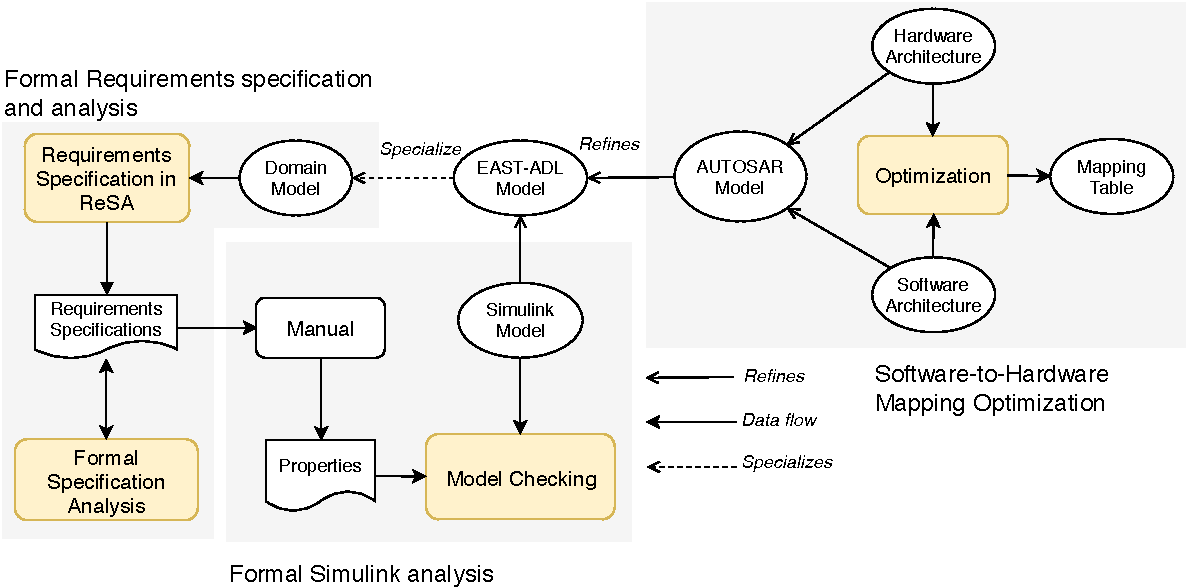
\includegraphics[width=\linewidth]{images/workflow}
	\else
	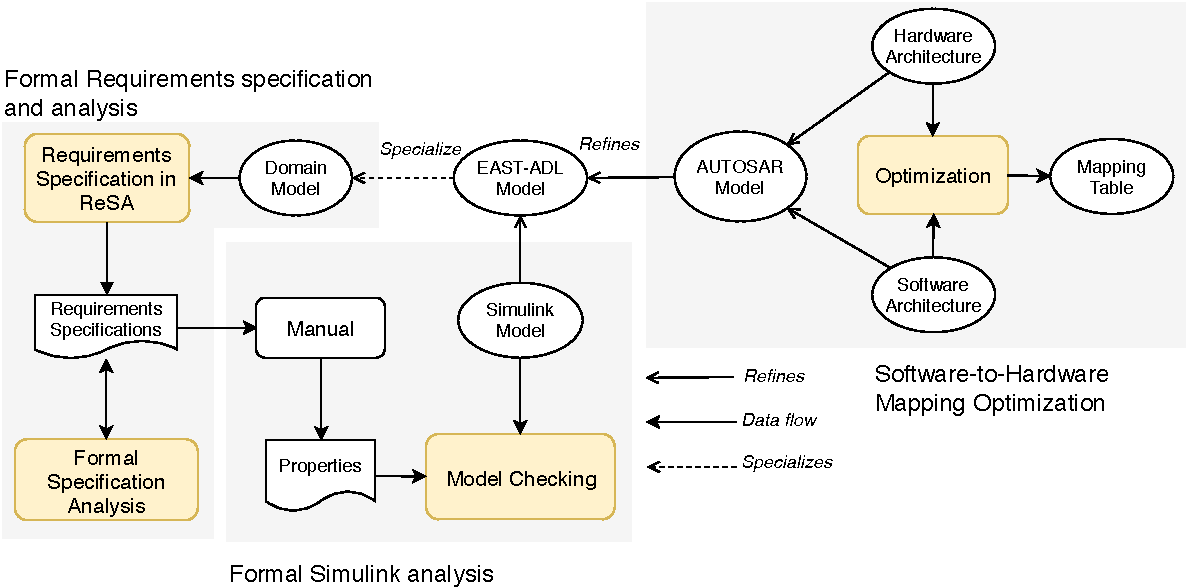
\includegraphics[width=.8\linewidth]{images/workflow.eps}
	\fi
	\caption{Thesis contributions workflow.} 
	\label{fig_workflow}
\end{figure}

Initially the textual requirements are specified in our domain-specific language \resa, which is a constrained natural language tailored to embedded systems. The \resa{} editor supports content completion as it is connected to a system model, which contains instantiations of words/phrases. If the \resa{} editor is required to be domain-specific, e.g., to the automotive domain that employs \eastadl, the system model is specialized to the latter model, thus enabling requirements specifications by accessing \eastadl{} model elements from the editor. To check the consistency, the \resa{} specifications are translated into Boolean and description logic, respectively, and subsequently analyzed via SAT solver and inference engine (or reasoner), respectively.

After the quality of the specifications is checked and improved if needed, that is made unambiguous, comprehensible, consistent, they can be used in the verification of behavioral software designs. In this thesis, we consider that the software design is created with Simulink, which is one of the most popular integrated environments for modeling, simulation and analysis of embedded system functions. In order to analyze a Simulink model rigorously, we transform it automatically into a formal model, specifically a network of stochastic timed automata. Subsequently, the latter is analyzed via statistical model checking against properties initially expressed in \resa, but manually translated into the query (properties) language of the model checker, that is probabilistic weighed-metric temporal logic (PWMTL).

At the architectural level, the Simulink model is represented by \eastadl{}, and at the implementation level by an \autosar{}, which consists of software components that communicate through a virtual function bus (VFB).  Note that, the refinement from the \autosar{} model to the Simulink model is manual, which is the normal practice, however, the Simulink model composition (or structure) is automatically generated. The software architecture complements the Simulink model with computation resource specifications, that is via runnables, which are schedulable pieces of code (or objects) by the \autosar{} OS. Moreover, AUTOSAR also complements Simulink models with resource specifications, such as power specification, interface specification of the underlaying hardware, etc. In this regard, we propose exact and heuristic software-to-hardware optimization techniques that incorporate the timing and reliability of software applications as constraints, and optimize the power consumption of the software.

The thesis contributions are summarized in the next sections. 
\section[RC1: {\sffamily \resa{}} -- \textbf{Re}quirements \textbf{S}pecification L\textbf{A}nguage]{RC1: \\{\sffamily ReSA} -- \textbf{Re}quirements \textbf{S}pecification L\textbf{A}nguage}\label{rc_resa}
We propose a domain-specific and constrained natural language, both at the syntax and semantics level, which is designed to improve comprehensibility and reduce ambiguity of embedded systems requirement specifications. The language employs concepts from the embedded systems domain, e.g., \textit{System}, \textit{Parameter}, \textit{Device}, \textit{State}, \textit{Mode}, \textit{Entity}, to typeset domain-specific words/phrases. Besides grammatical rules (or syntax), semantic relations between the concepts limit the possible construction of the specifications. For instance, the sentence``The ASL shall limit the driver.'' is a grammatically-correct specification, but semantically it makes no sense. To solve this problem, the \resa{} type system imposes a type constraint on the relation between instances ``The ASL''\textit{:system} and ``the driver''\textit{:user}.

\subsection*{Syntax}
The language design is modular, in the sense that it uses sentence categories, e.g., \textit{Simple}, \textit{Compound}, to structure the specifications, thus improve comprehensibility and reduce ambiguity. It also allows complex specifications by inductively applying the grammar rules of the language. The following context-free grammar is a snippet of the \resa{} language. 
\begin{bnf*}
	\bnfprod{specification}
	{\bnfpn{simple} \bnfor \bnfpn{complex}\bnfor\bnfpn{nested-complex} ...}\\
	\bnfprod{simple}
	{\bnfpn{mainClause} .} \\%\bnftd
		\bnfprod{complex}
	{\bnfpn{subClause}, \bnfpn{mainClause}.} \\%\bnftd
	\bnfprod{mainClause}
	{\bnfpn{primitiveClause}\bnfor ...} \\%\bnftd
		\bnfprod{primitiveClause}
	{\bnfpn{sub} \bnfpn{verb} \bnfpn{obj}\bnfor...} \\%\bnftd
	\vdots
\end{bnf*}
For the detailed grammar specification of the language, the reader is invited to refer to Paper~A~\cite{Mahmud2015ReSA:Systems} and its documentation
\footnote{ReSA documentation:  \url{https://bitbucket.org/nasmdh/resa/src/master/} }
\begin{example}[Adjustable Speed Limiter (ASL) Requirements]\label{ex_resa_example}
	We here give an example of selected requirements of the ASL system, which is a speed control system found in Volvo trucks. It controls the vehicle speed to not exceed a certain speed, which is set by the driver or legal authorities. It consists around 300 fuctional and extra-functional requirements. Just to demo the usage of the language, we specify only four of ASL equirements.
\begin{elaboration}{0.95}
	\small
		\begin{tabular}{lp{.9\textwidth}}
			R1 & ASL:system shall send "the driver"\textit{:user} notification:status every 200ms. \\
			R2 &\begin{tabular}[t]{@{}l@{}}if ``driver:user'' selects ``ASL speed control''\textit{:mode} and\\
				\hspace{0.5cm}(vehicle is in ``pre-running'' mode or
				vehicle is in ``running'' mode)\\ then\\
				\hspace{0.5cm}ASL:system shall be enabled within 200ms and\\
				\hspace{0.5cm}``ASL enabled''\textit{:status} shall be presented to ``the driver''\textit{:user} \\ endif\end{tabular} \\
			R3 & After ASL:system is enabled, if IncButton\textit{:inDevice} is pressed, ASL:system shall be activated.\\
			R4 &if driver selects ``ASL speed control''\textit{:mode}
			then 
			ASL\textit{:system} shall be disabled.
		\end{tabular}
\end{elaboration}
\end{example}

\subsection*{Tool Support and Validation on Adjustable Speed Limiter}
The \resa{} language is implemented~\cite{resatool} in the Xtext framework\footnote{\url{Xtext: https://www.eclipse.org/Xtext/}}, which is an Eclipse-based integrated development environment for the development of domain-specific and general-purpose languages. The \resa{} editor, which is shown in Figure~\ref{fig_resagui}, supports content completion, errors/warring messages and boilerplate management. The editor is integrated in \eatop, meaning that the editor can be triggered from within the IDE, moreover, the content-completion feature displays contents of the \eastadl{} model elements, hence enabling the consistent use of vocabularies during specification. The \resa{} tool as a standalone, and as a plugin for \eatop{}, can be downloaded from the URL {\small \url{https://bitbucket.org/dashboard/overview}}. 
\begin{figure}[h]
	\centering
	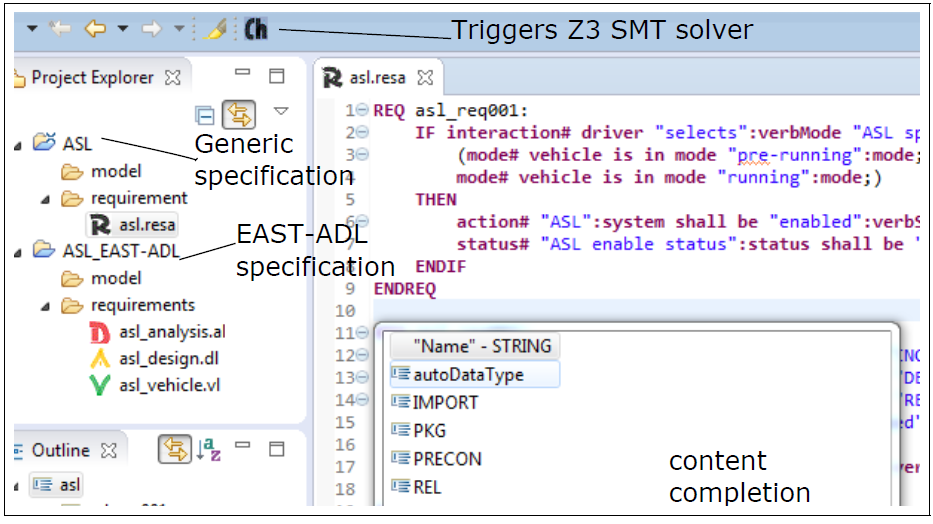
\includegraphics[width=1\linewidth]{images/resagui}
	\caption{The \resa{} graphical user interface (GUI).}
	\label{fig_resagui}
\end{figure}

The language as well as its tool support is validated on the 300 ASL requirements, which are initially expressed in natural language. The requirements distribution is as shown in Figure~\ref{fig_ASLreqs}, in terms of types of requirements. The requirements are rewritten in \resa, and Figure~\ref{fig_ASLreqsresult} shows the sentence categories (or boilerplates) employed to specify the requirements. In general, the language is expressive, though it is constrained, and is extensible with constructs that improve its expressiveness.
 \begin{figure}[h] 
 	\centering
 	\subfloat[Types of ASL Requirements.\label{fig_ASLreqs}]{% 
 		\centering
 		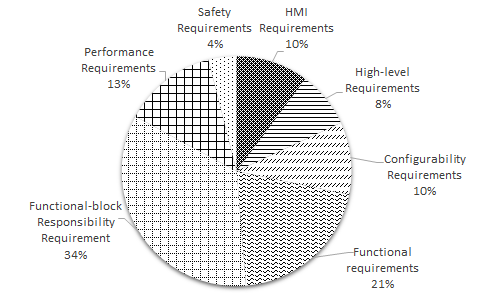
\includegraphics[width=0.45\textwidth]{images/aslreq}
 	} \hfill
 	\subfloat[Distribution of ASL boilerplate types.\label{fig_ASLreqsresult}]{% 
 		\centering
 		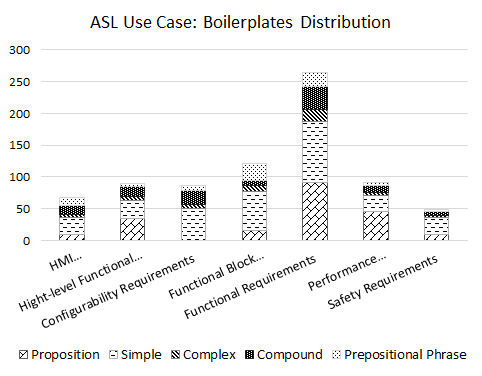
\includegraphics[width=0.45\textwidth]{images/aslbp} 
 	} 
 	\caption{Specifying ASL requirements in \resa.} \label{fig_resa_asl}
 \end{figure}
\section[RC2: Consistency~Checking of {\sffamily ReSA}~Specifications]{RC2: \\Consistency Checking of {\sffamily ReSA} Specifications}\label{rc_resaanalysis}
The editor shows syntax and typing warning and error messages. However, such static analysis is rudimentary and is per specification. In this contribution, we propose two methods of consistency analysis: \textit{SAT-based} analysis and \textit{ontology-based} analysis, which analyze over multiple specifications.

\subsection*{SAT-based Analysis}
Boolean satisfiability (also known as SAT) can informally be defined as the problem of finding truth values (or assignments of Boolean variables) such that a Boolean formula holds. It is NP-complete, however, there exist efficient heuristic algorithms that solve SAT problems of large size, e.g. with thousands of Boolean variables. Therefore, we first transform the \resa{} specifications into Boolean expressions~\cite{resatool}, then we formulate the problem of finding inconsistencies of the Boolean expressions, in terms of SAT as follows:
\begin{definition}[Inconsistency of Specifications]
	Let $\Phi = \{\Phi_1, \Phi_2,\dots,\Phi_n\}$ be the \resa{} specifications and after translating its constituents into Boolean expressions,  $\phi_i, i \in [0,..,n]$. Consequently, $\phi_1, \phi_2,...,\phi_n$ are Boolean formulas, each denoting a requirement respectively. We say that the set of Boolean formulas $\phi$ is \textit{inconsistent} if the expression $\phi_1 \land \phi_2 \land\dots\land \phi_n \Rightarrow false$ holds, that is, there exists at least one expression that cannot be satisfied:  $\exists i. \phi_i |= false$. 
\end{definition}
\begin{example}
Assume that we want to check the consistency of the requirements that are specified in Example~\ref{ex_resa_example}. Figure~\ref{fig_z3} shows the translation of the specifications into Boolean expressions (in Z3  SMT-LIB format). Each expression is asserted before the Z3 solver is called using the command $(check-sat)$. Some clauses are resolved for negation and opposite words, e.g., the fact that ``enabled'' is opposite of ``disabled'' implies $p_5=p_7\neq p_{11}$. The solver returned ``\textit{unsat (R2 R4 R1\_Assertion)}'',  which means, the expressions are inconsistent and indicates the specifications that are responsible for the inconsistency (or unsat-core).
\end{example}
\begin{figure}[h]
	\centering
	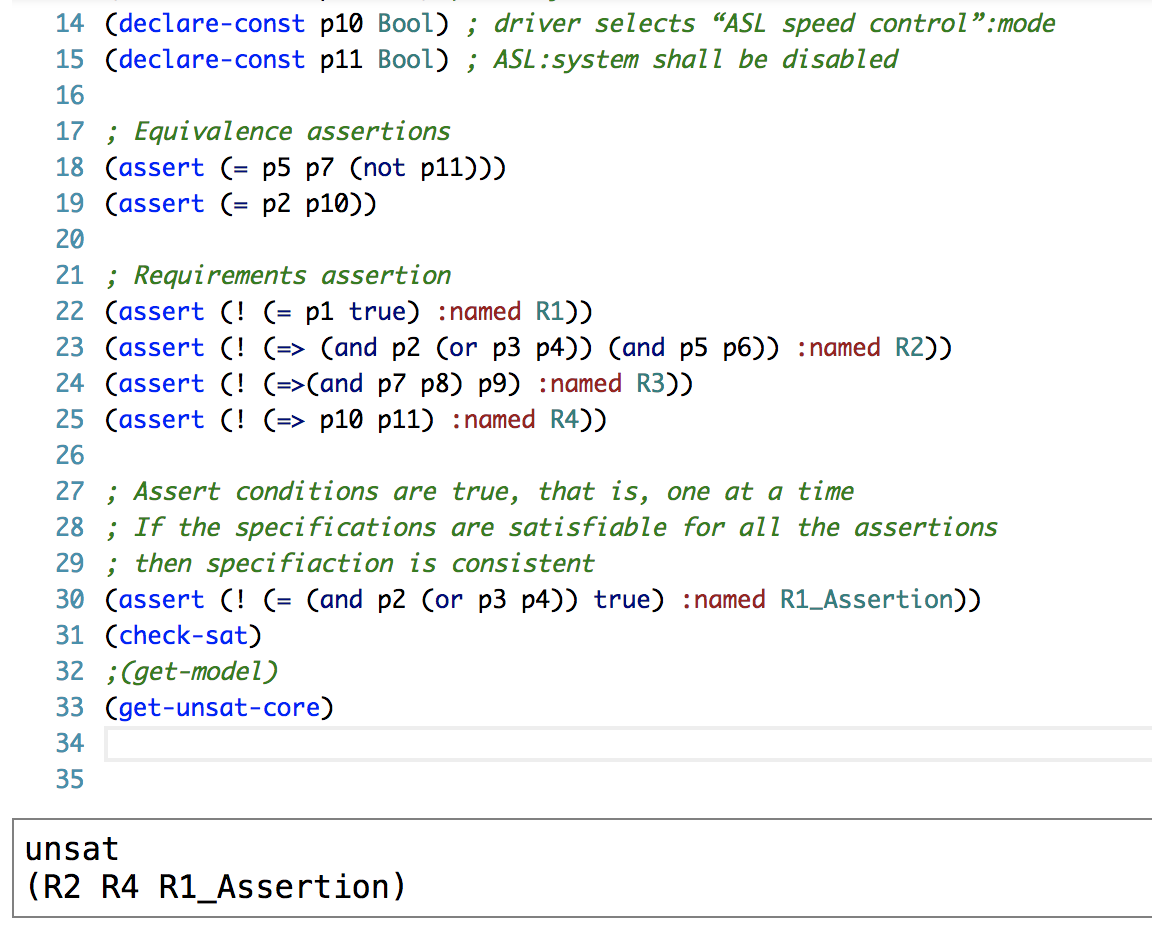
\includegraphics[width=0.7\linewidth]{images/z3}
	\caption{The \resa{} specifications R1 - R4 encoded as Z3 format, and the unsat-core feedback from the Z3 solver, to localize the source of the inconsistency.}
	\label{fig_z3}
\end{figure}

The SAT-based analysis, although easy and scalable, does not allow rigorous analysis. This is due to the fact that the Boolean (or propositional) variables abstract away details of the clauses in the specifications. %The ontology-based approach solves this problem with trade off over scalability.

\subsection*{Ontology-based Analysis}
\textit{Ontology} as a knowledge representation technique can be used to capture the intricate relations of words/phrases of specifications, for instance, synonyms, antonyms, generalization. Moreover, it can be used to capture the syntax of the specifications as well, essentially modeling the \resa{} specification as a concrete requirements specification ontology. 

Besides the challenge of constructing the ontology, accurate representation of the specifications is crucial to a certain degree for the ontology to be useful, that is, the specifications should be interpreted linguistically. In this research, we propose the \textit{event-based} semantics approach~\cite{Mahmud2017SpecificationLogic} to construct the meaning of each specification compositionally from its constituents (or grammar units). The event-based semantics, which is based on the first-order logic, uses an existentially-quantified events to relate words/phrases (or arguments of predicate) , clauses, adjuncts of a sentence~\cite{Mahmud2017SpecificationLogic}. To help intuition, let us assume the following example: the clause ``ASL:system shall limit ``vehicle speed'':parameter'' is represented as $\exists e$[limiting($e$) \& Agent(ASL) \& Recipient(vehicle speed)], where Agent and Recipient are known as \textit{thematic} roles, which define the semantic roles of the arguments in the clause.  Since the requirement specifications entail technical words/phrase, the thematic roles of these arguments are not obvious, so we extended the thematic roles into the \resa{} concepts, in this way, the interpretation of the clauses becomes domain-specific, for example, classifying instances of \textit{System} or \textit{User} as \textit{Agent}, and  instances of \textit{Parameter} as \textit{Recipient}.  

Following the event-based semantics, the \resa{} specifications are translated into description logic as ontology. Once the ontology is constructed considering the event-based semantics, thematic roles, lexical relation, we check its consistency via an inference engine (or reasoner), which is a software program that applies logical rules on a logical system, such as the ontology, to obtain new information.
\begin{definition}[Inconsistency of Specifications]
	The requirements specification ontology is inconsistent if there does not exist an interpretation (or a model) $M$ that satisfies the terminological assertions $T$ and the concrete assertions $A$, that is, $M \not\models ax$, where: $ax \in T \cup A$, where $T$ is a set of terminological assertions and $A$  a set of facts (or concrete assertions).
\end{definition}

\section[RC3: Statistical~Model~Checking~of~Simulink Models]{RC3: \\Statistical~Model~Checking~of~Simulink Models}\label{rc_sim}
Several research endeavors do exist on the topic of formally analyzing Simulink models. Some of them are using theorem proving, others exact model checking and others statistical model checking. Many of the proposed solutions are  limited either due to frequent user involvement or scalability issues. In this thesis, we propose a scalable formal analysis of large-scale Simulink models via statistical model checking. The Simulink models can be discrete, continuous or hybrid, moreover, they can consist of atomic and composite Simulink blocks that are scattered on multiple files, which is a practical scenario. Essentially, we consider typical industrial Simulink models, e.g., the Brake-by-Wire and Adjustable Speed Limiter Simulink models from VGTT~\cite{Filipovikj2018SimppaalModels}.

To enable statistical model checking of Simulink models, we first define the syntax and semantics of blocks and their composition, in terms of timed transition systems. After that, we transform the Simulink blocks of a model, after flattening, in networks of stochastic timed automata that can be model checked statistically with \uppaalsmc.  Our approach has the following important characteristics: (i) the transformation employs continuous and discrete transformation patterns, which are generic and reusable, thus can be applied to any Simulink blocks; (ii) the transformation preserves the execution order of Simulink blocks; (iii) it is robust, meaning that, it handles various models such as continuous, discrete, hybrid, and models that contain blocks with with different sampling rates, also known as multi-rate blocks.

\subsection*{Transformation Patterns} 
The continuous-time and discrete-time stochastic timed automata (STA), which are shown in Figure~\ref{fig_patterns}(a) and \ref{fig_patterns}(b), are used to transform the continuous-time and discrete-time Simulink blocks into their respective STA. In both cases, the automata traverse the respective edges from the ``Start'' locations to the ``Operate'' locations, respectively, at the global time $sn*IAT$, which is determined according to each block's order of execution $sn$, that is, the lower $sn$, the sooner the automaton moves to the ``Operate'' location, and $IAT$ is an infinitesimal inter-arrival time between subsequent executions of the automata. In case of the continuous-time STA pattern, the automaton loops at the ``Operate'' location every infinitesimal sample time, which is distributed exponentially according to the rate  $\lambda=1000$. In the discrete-time STA pattern, the automaton loops at location "Operate" every $ts$ sample time with probability 1, as there is only one edge that goes out of the location and the delay transitions are distributed uniformly in the interval $[ts,ts]$.
\begin{figure}[h] 
	\centering
	\subfloat[Continuous-time.\label{fig_continuous}]{% 
		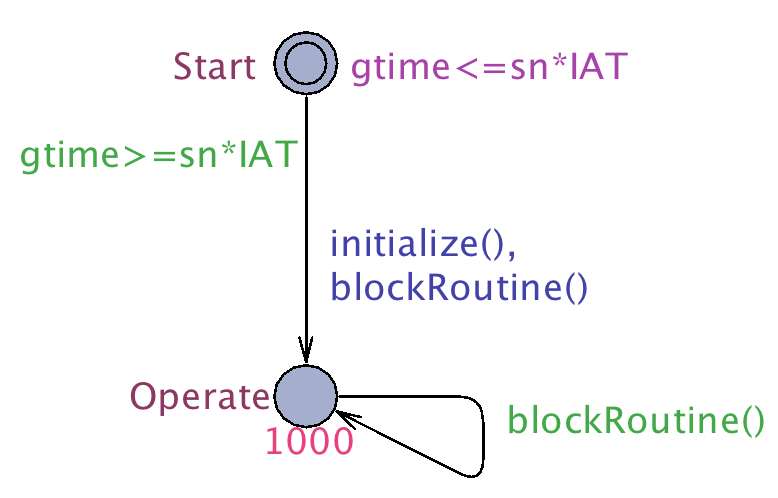
\includegraphics[width=0.45\textwidth]{images/continuous-sta}
	} ~
	\subfloat[Discrete-time.\label{fig_discrete}]{% 
		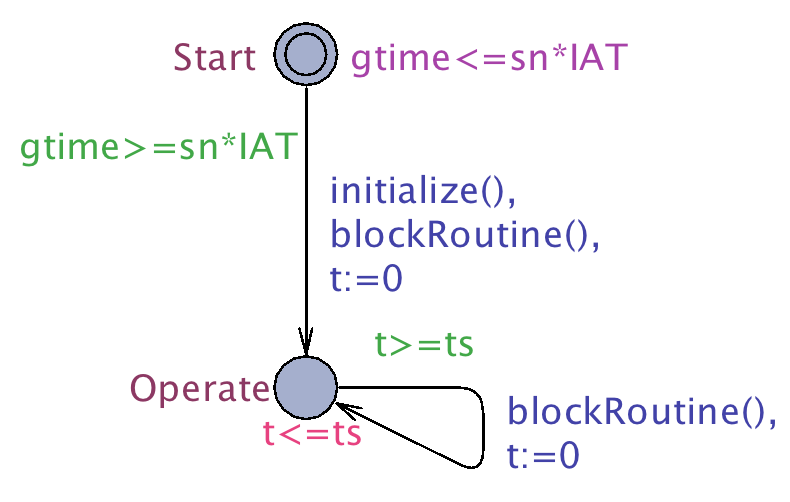
\includegraphics[width=0.45\textwidth]{images/discrete-sta}
	} 
	\caption{STA transformation patterns.} 
	\label{fig_patterns}
\end{figure}

\subsection*{Simulink to NSTA Transformation Process} 
Besides proposing the transformation patterns, we provide an automatic transformation of a Simulink model to its equivalent network of STA by applying the following tasks:
\begin{enumerate*}[label=(\roman*)]
	\item the Simulink model is simulated, subsequently, the sorted-order list, which contains the execution order of the Simulink blocks, is extracted;
	\item in case the model is hierarchical, the execution order is flattened first, thus generating a flattened sorted-order list;
	\item the Simulink model is parsed, as a result, each block is translated into a stochastic timed automaton via the corresponding transformation pattern. The sorted-order number $sn$ is instantiated from the sorted-order list on the fly;
	\item any non-computation blocks is accounted in the transformation but is not transformed into an automaton; examples of such blocks are Mux, SubSystem blocks etc.;
	\item the connections between the blocks are translated into global variables, which act as the communication means between the automata.
\end{enumerate*}
For details on the transformation, as well as on the soundness proof for discrete-time models, the reader is invited to consult Paper D~\cite{Filipovikj2018SimppaalModels}

%\begin{figure}
%	\centering
%	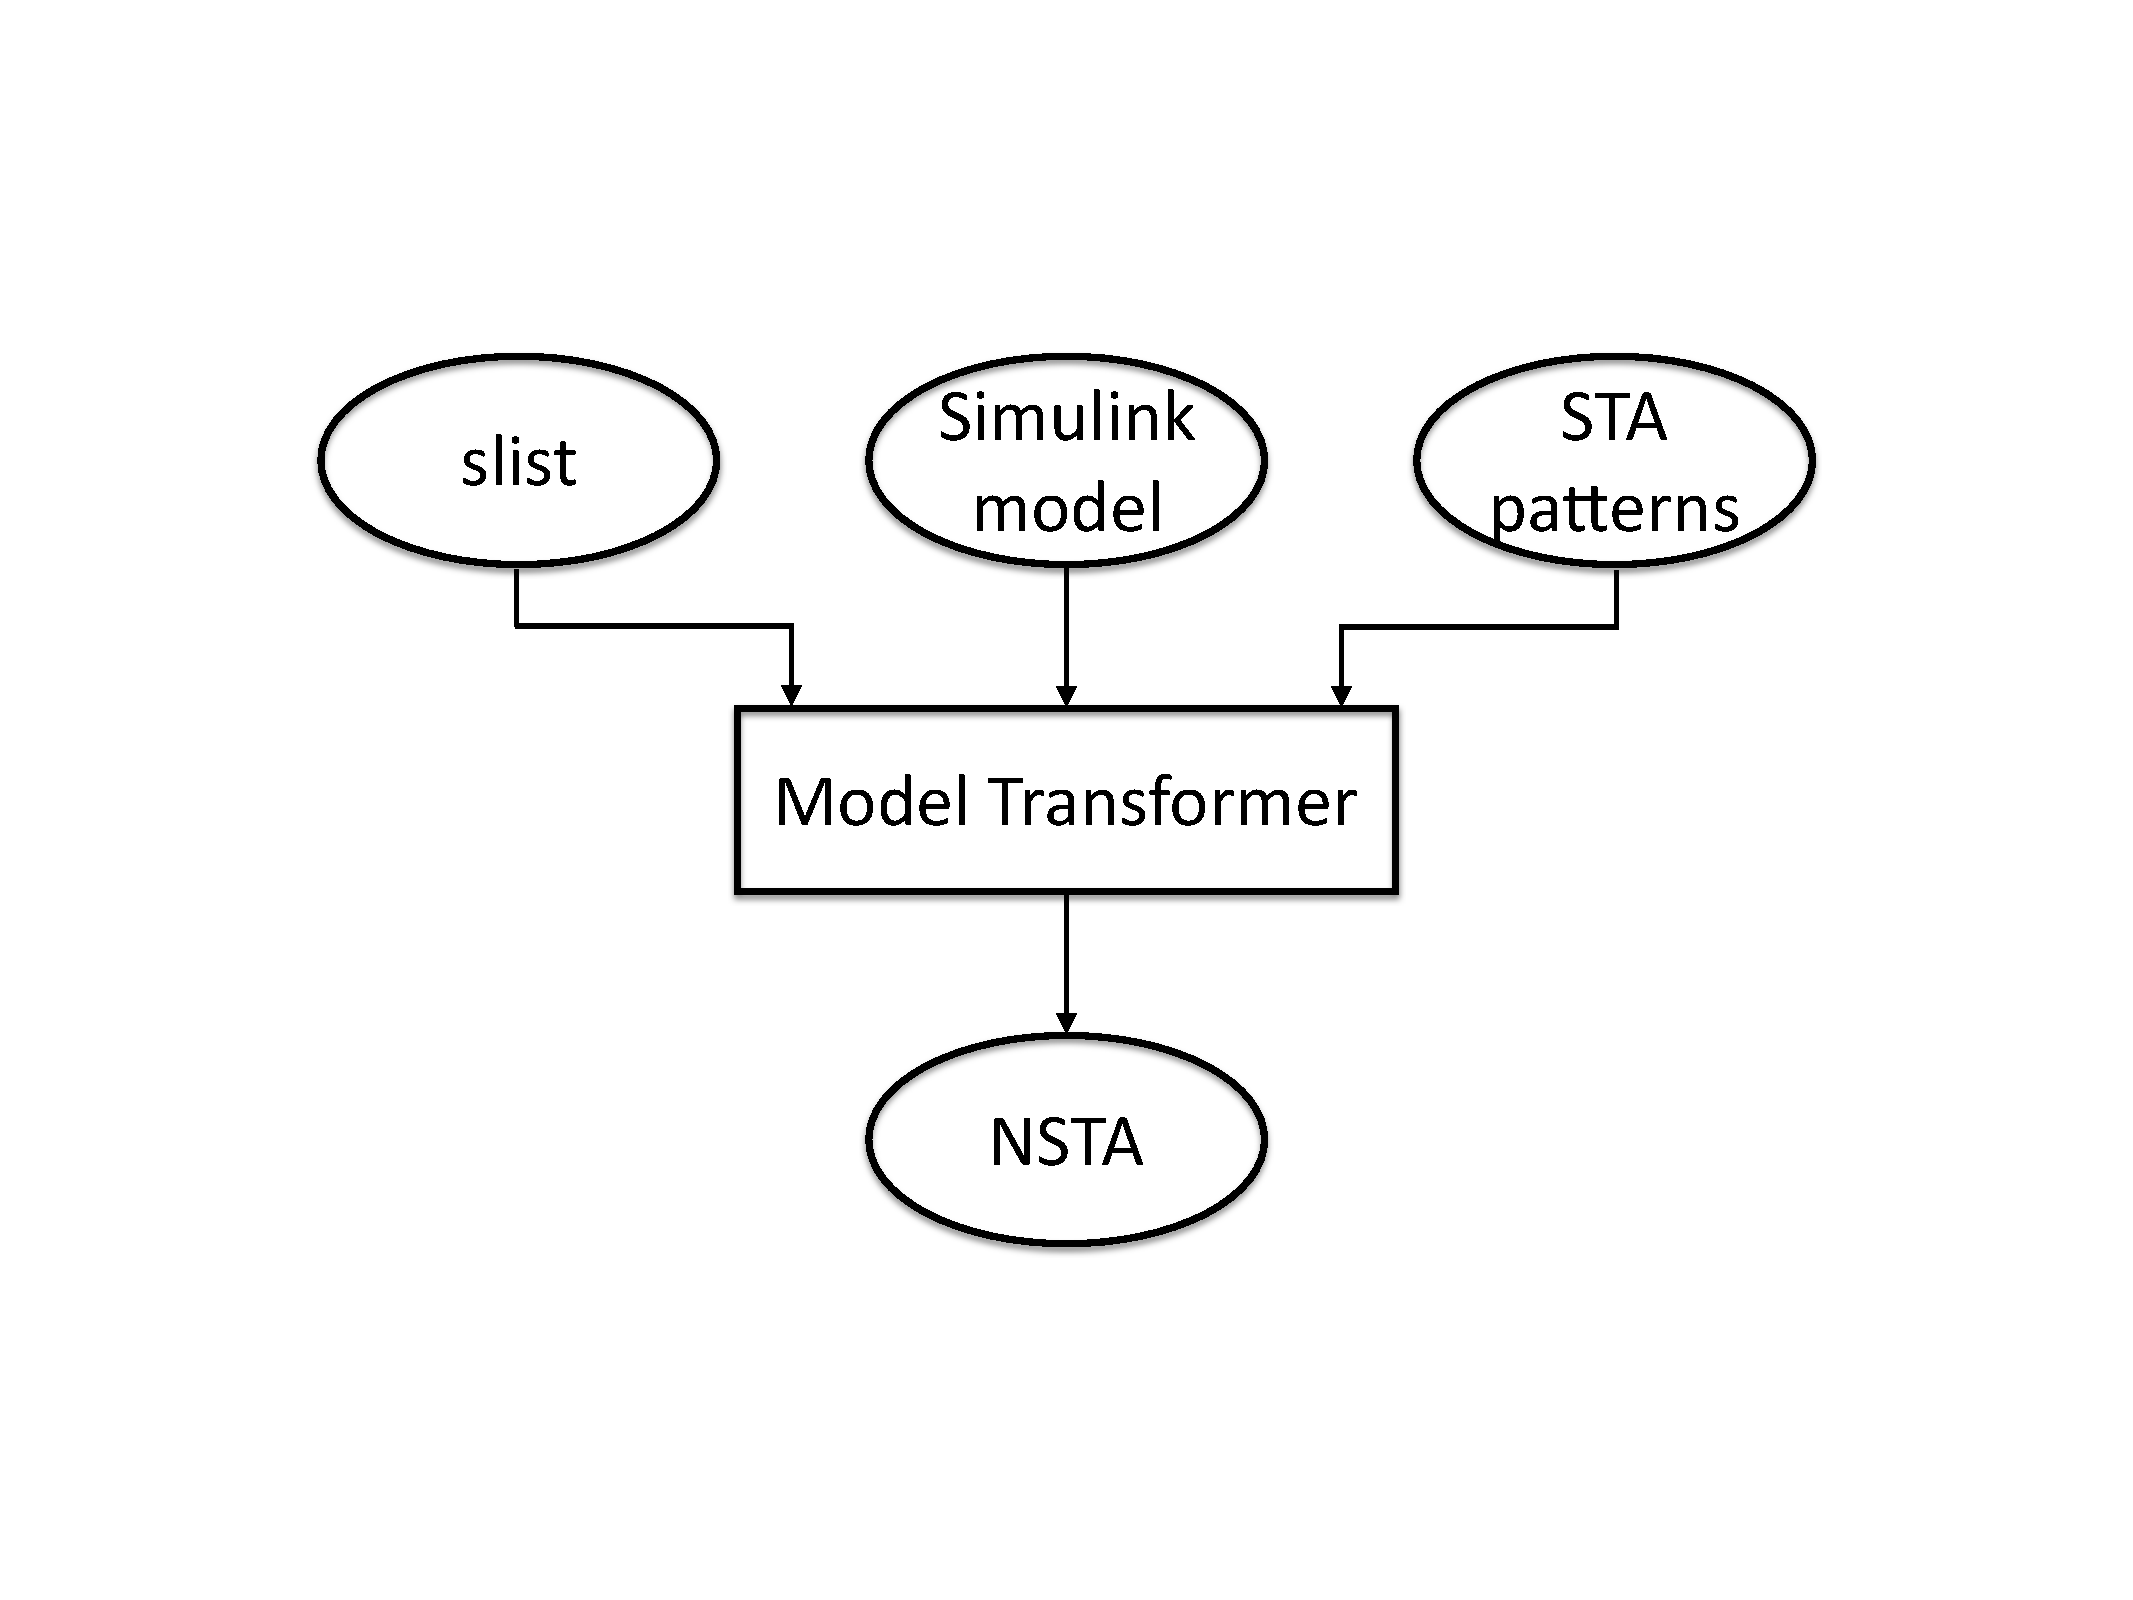
\includegraphics[width=0.6\linewidth]{images/simulinkapproach}
%	\caption{Simulink to NSTA Transformation}
%	\label{fig_approachworkflow}
%\end{figure}

\subsection*{Validation on the Brake-by-Wire Use Case} 
Our approach is applied on an industrial Brake-by-Wire Simulink model, which is a prototype developed for academic use by VGTT. The model consists of 320 blocks, of which 19 are discrete blocks, 26 constant blocks and the rest are continuous blocks. The model design consists of modules that collect sensory data, e.g., vehicle speed, pedal position, and compute the proportional torque force that is applied on the wheels to brake the vehicle. Besides, it has the  anti-braking functionality (ABS) to avoid (or minimize) skidding, which occurs when the slip rate of a wheel is greater than its friction coefficient. 

The BBW requirements are initially specified in \resa, subsequently are translated into PWMTL properties manually by using monitors (or observers), which are stopwatch stochastic priced timed automata. The monitors are modeled for particular requirements, and basically observe the progression the execution of the automata.
\begin{example}[Statistical model checking of BBW]\label{ex_resa}
	The BBW model is automatically transformed into a network of STA, and we model monitors~\cite{Filipovikj2018SimppaalModels} to represent 5 functional and timing requirements, out which 3 requirements are shown in the box below for illustration. 
	\vspace{0.2cm}
\begin{elaboration}{0.9}
	\small
	{}
	\begin{tabular}{lp{.85\textwidth}}
	R1 & The brake request shall be computed within 10 ms. \\
	R3 & The brake request shall be propagated to two different wheel actuators within 4 ms.\\
	R4 & If the brake request is 0, then the ABS shall set the torque to 0. \\
\end{tabular}
\end{elaboration}
\end{example}

Figure~\ref{fig_smcresult} shows the PWMTL properties and their model-checking results. R1 and R3 as presented in the able above  are safety requirements expressed using the $\Box$ (always) operator in their formal counterpart, as indicated by R1$_{BBW}$ and R3$_{BBW}$ PWMTL properties of Figure~\ref{fig_smcresult}. R4 is a conditional requirement expressed using the $\Diamond$ (eventually) operator in its formal translation, as encoded by the R4$_{BBW}$ PWMTL property. Each result in Figure~\ref{fig_smcresult} shows the probability interval of satisfying the property (qualitative), confidence level, the number of runs and the time needed by the model checker to return the result. For some properties in Table~\ref{fig_smcresult}, the probability interval of satisfying the respective property is $[0.99, 1]$, which can be considered as ``property satisfied'' if the lower bound on the probability is 0.99. However, in many safety-critical applications, the requirement on the probability is normally high, e.g., 0.999999 (essentially approximates to ``no failure should happen''). In this case, the interval should be more precise, which can be achieved by lowering $\alpha$ and $\beta$ of the hypothesis testing, which are probabilities of accepting false positives, and false negatives, respectively~\cite{David2011StatisticalAutomata}.
\begin{figure}
	\centering
	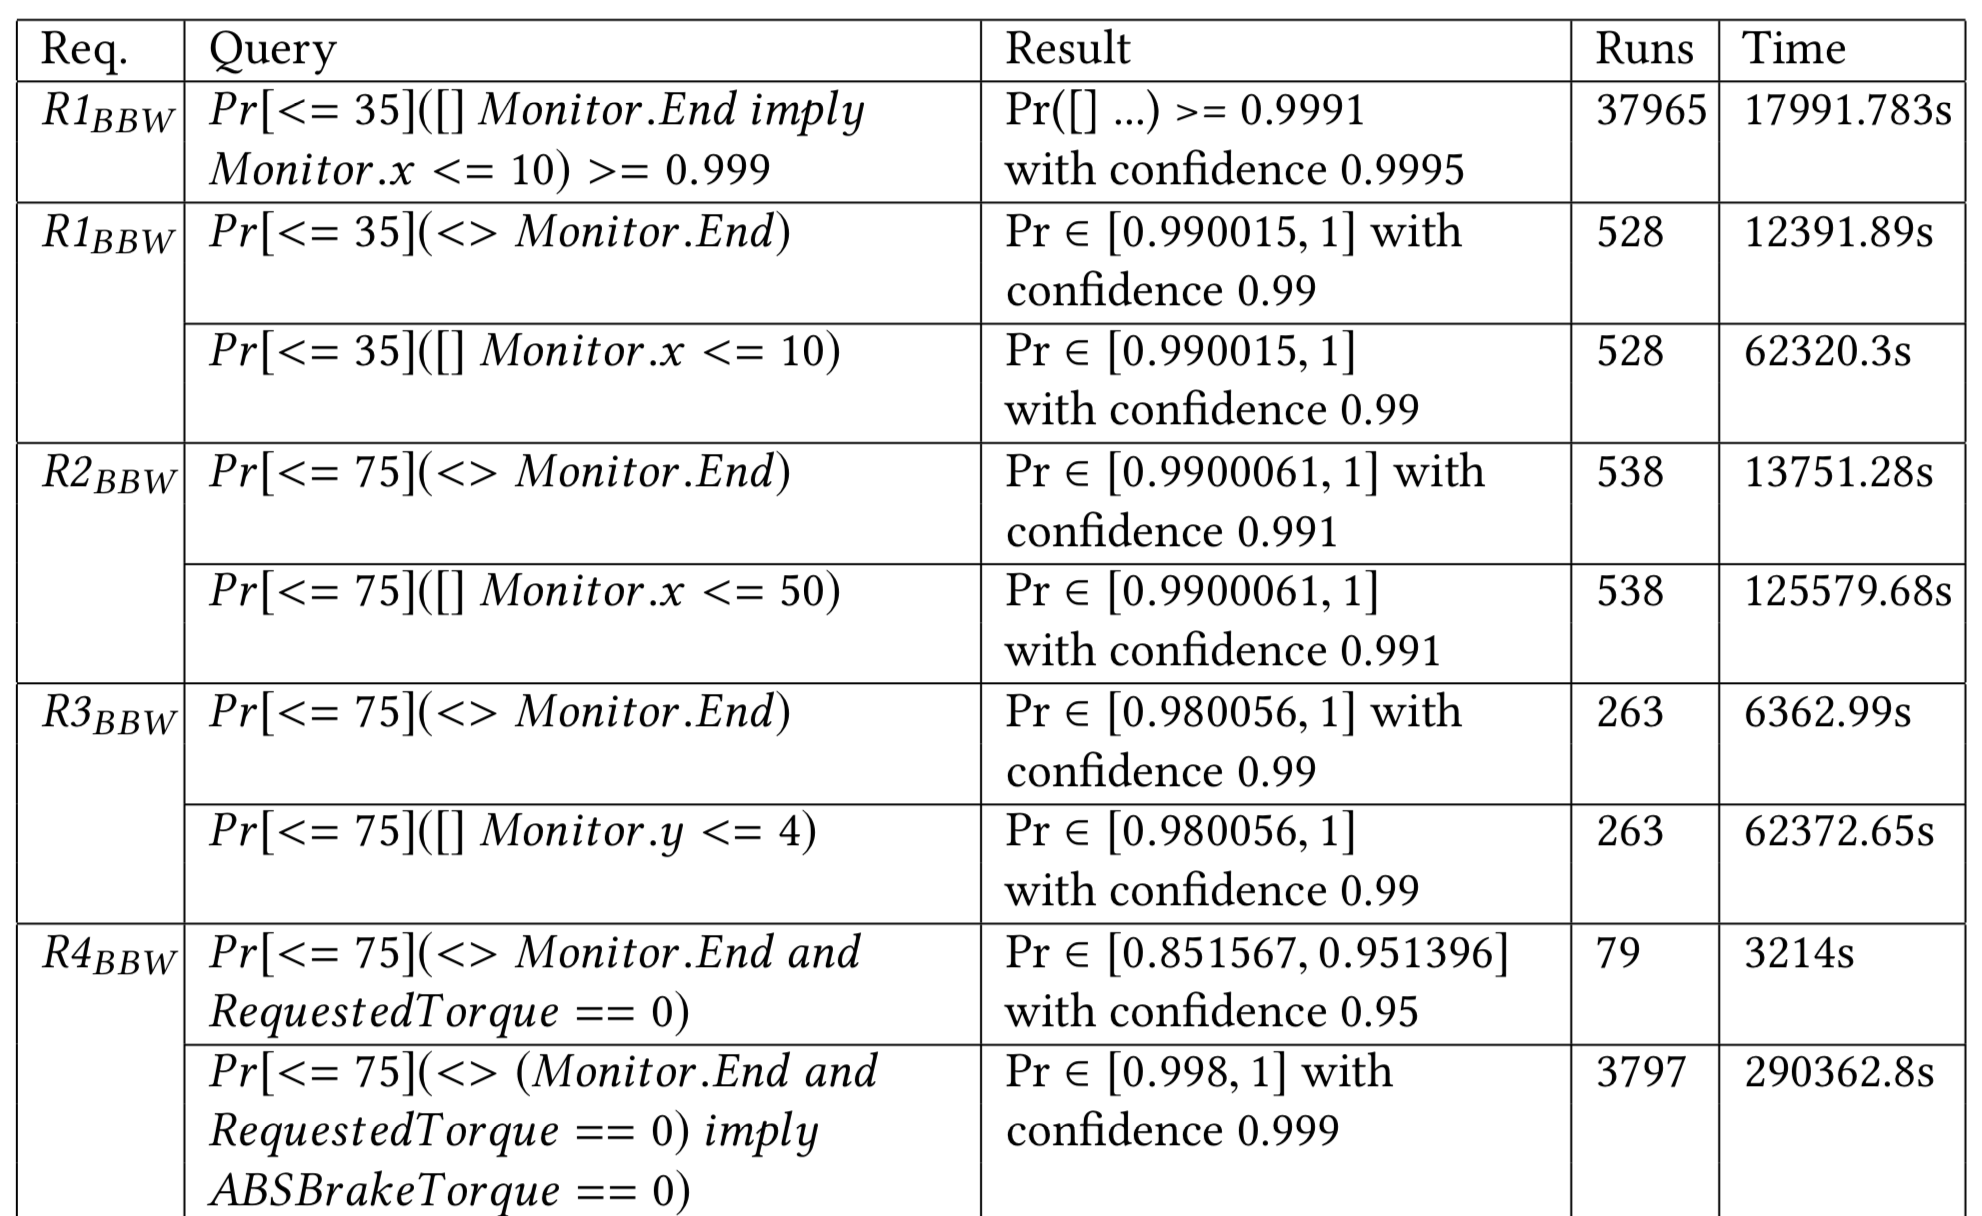
\includegraphics[width=1\linewidth]{images/smc_result}
	\caption{Analysis results snippet of the BBW Simulink model from \uppaalsmc{}. For the complete results, we refer the reader to~\cite{Filipovikj2018SimppaalModels}.}
	\label{fig_smcresult}\vspace{-0.2cm}
\end{figure}

\section{RC4: Fault-tolerant Software Allocation}\label{rc_ilp}
In this thesis, we have proposed two software allocation approaches based on integer linear programming (ILP) and hybrid  particle swarm optimization (PSO) optimization algorithms. The system model is briefly described as follows. We consider an \autosar{} safety-critical software application that can be mapped to multiple computing nodes, which are heterogeneous with respect to power specification, failure rate and processing speed. The software application has end-to-end timing and reliability requirements, which must be satisfied by the mapping solution. In order to meet the reliability requirement, the allocation applies fault tolerance by replication of software components, which are mapped to different computing nodes. We assume the nodes failures are mutually exclusive and permanent, and the replication is active, hence no time between failures is assumed.

The software application is modeled as directed acyclic graph (DAG), where the nodes are runnables and the links are communications between the runnables. A cause-effect chain (or chain) is a sequence of runnables that realize some software functionality, e.g., the pressing of a brake pedal (the cause) and the slow down of a vehicle (i.e., the response). Before the allocation begins, the runnables are mapped to tasks using merging rules according to the \autosar{} methodology. The tasks and messages that realize the safety-critical software functionality are scheduled using a fixed-priority preemptive scheduling policy~\cite{Sha2004RealPerspective} and fixed-priority non-preemptive scheduling policy (over a  CAN bus), respectively. We assume that the runnables are triggered periodically and have multiple worst-case execution times for the different processors.

\subsection*{Allocation via Integer Linear Programming}
Consider that the mapping solution is represented by a vector of binary matrices $\textbf{x}=\{\textbf{x}_1:1,...,K\}$, where \ttxkij{} represents the mapping of the software component $q^{k}_{ij}$ to the computing node $\ssb{n}[j]\in \mathcal{N}$. 
\begin{equation}
\label{eqn_solution}
\bspx{k}=
\begin{bmatrix} 
\ssx{k}{11} & \ssx{k}{12} & \dots & \ssx{k}{1K}\\
\ssx{k}{21} & \ssx{k}{22} & \dots & \ssx{k}{2K}\\
\vdots & \vdots & \ddots & \vdots\\
\ssx{k}{N1} & \ssx{k}{N2} & \cdots & \ssx{k}{NK}
\end{bmatrix}
\end{equation}

The power consumption of a software application that is mapped to computing units $N'\in N$ is calculated as the sum of the power consumption of each node $n_h\in N'$, i.e., $\mathcal{P}_{total}(x)=\sum_{n\in N'}{\mathcal{P}(u_n(x))}$, where $\mathcal{P}(u)$ is the power consumption of a computing node which is linearly proportional to its utilization~\cite{Mahmud5222}. The utilization of a computing node is the sum of the utilization of its constituent tasks (or software components). Equation (\ref{eqn_isp_util}) computes the utilization of the nodes.
\begin{align}
\label{eqn_isp_util}
	(u_1,...,u_K)(\x)=\sum_{k=1}^{K}\sum_{\tau\in T_{c_i}}{\xkij*\frac{C_\tau}{P_\tau}},
\end{align}
where $T_{c_i}$ is the set of tasks which realize the software component $c_i$ (which is a type for $q^{k}_{ij}$ replica), $C_\tau$ and $P_\tau$ are the worst-case execution time and  period of the task $\tau$, respectively.

We apply the classical worst-case response time analysis~\cite{Baruah2011Response-timeSystems} to check the schedulability of tasks sets in each node. The analysis is recursive, and depends on a higher priority tasks set, which is dynamic for different mappings. The end-to-end delay of a chain is calculated for data age (also known as age delay), which is iterative. Thus, we propose a formulation of the timing constraints as logical linear constraints as follows: (i) we identify the the software components partitions $P=2^C$, where $p\in P$ can be mapped to a node; (ii) we check the schedulability of each partition in each node $Y_j=\{p\in P| isSched(p,n_j)\}$, where $sched$ is a Boolean predicate that returns \textbf{true} if $p$ is schedulable on $n_j$.  A partition is identified by a sequence of 0s and 1s based on its constituent components, e.g., the id of the partition $\{c_1,c_4,c_5\}\subseteq \{c_1,c_2,c_3,c_4,c_5\}$ is $10011=19$. So, given the mapping $\x$, the partition id that is mapped to the computing node $n_j$ can be computed as
\begin{align}
	g_j(\x)=\sum_{i=1}^{N}{10^{N-i}\max_{1\leq k< K}\xkij}
\end{align}
where the $\max_{1\leq k< K}$ function returns 1 if at least one component replica is mapped to $n_j$ otherwise returns 0, indicating no replica is mapped to that node. Thus, each node must have a valid partition that is schedulable as indicated in the logical constraint,
\begin{align}
\bigvee\limits_{p\in Y_j}g_j (\x)= id(p) ,
\end{align}
where $id(p)$ is a predicate that returns the id of the partition $p$.

Similar to the tasks deadline constraints, we construct logical constraints that correspond to the valid set of chains. Given $\Gamma =\{\Gamma_i:i=1,...,N\}$ chains, the set of possible mappings of each chain $\Gamma_i$ on a set of $\mathcal{N}$ nodes is ${\Gamma_i}^\mathcal{N}$. Thus, the set of valid mappings of each chain that satisfy the end-to-end timing requirements are $Z_i=\{\gamma\in {\Gamma_i}^\mathcal{N}| ageDelay(\gamma) \leq {EE}_\gamma$.

The reliability constraint refers to the probability that the application functions by the time $t$, i.e $[0,t]$~\cite{Goel1985SoftwareApplicability}. % We assume that the reliability requirement of a software application is 0.99999999 over a 2-year operation time, which is to say  that the safety-critical system almost should not fail within the stated period. Furthermore, we assume that the mean-time to failure of the computing nodes is given as $10^6$ hours (0.0000001 per hour), which is the usual practice in many functional safety design.
Unless the the software application is replicated on one or more computing nodes, the reliability requirement is usually unattainable. So, the allocation strategy is basically to replicate sufficient software components to meet the requirement. However, the reliability calculation is not trivial as the replication results in functional inter-dependency of the computing nodes due to the replication of components, in which case, the series-parallel method does not always apply. Instead, we propose an exact method based on state enumeration~\cite{Lucet1999ExactReliability} of the computing nodes, i.e., all the possible configurations of the nodes $PS$ are enumerated. Subsequently, the reliability of the application is computed as the total probability of those configurations that allow functioning of the application~\cite{Mahmud5222}.
%, which is defined by its inverse as follows:
%\begin{definition}[Software Application Failure]
% 	A software application fails in the configuration $s\in\xi$ if there exists a component type $c_i$ where all of its replicas $Q_i$ \textit{fail}, otherwise, it functions, as determined by Equation (\ref{eqn_appreliability_milp_components}) using the floor function. The component replica $q_{ij}\in Q_i$ of type $c_i$ fails if $n_h$ fails, that is $s_h=0$. For instance, $s=101$ denotes the nodes $n_1$ and $n_3$ functions and node $n_2$ fails. 
% \end{definition}
% \begin{align}
% f_s(x) = \floor[\Bigg]{\frac{\sum_if_{c_i}(x,s)}{N}}=
% \begin{cases}
% 1 & \mbox{if } application \mbox{ functions}\\
% 0 & \mbox{if } application \mbox{ fails}
% \end{cases}\label{eqn_appreliability_milp_components}
% \end{align}h

% Thus, the reliability of the software allocation is
% \begin{align}
% \label{eqn_appreliability_milp}
% Reliability(\x)=\sum_{s\in PS}f_s(\x)*p_s,
% \end{align}
% where $p_s$ is the probability that the computing nodes attain a configuration $s$ which is computed as $p_s=\prod_{m\in M}\big[(z_m*\lambda_m) + (1-z_m)*(1-\lambda_m)\big]$, where $z_m\in\{0,1\}$ indicates if the node fails (i.e., 0) or functions (i.e., 1), $\lambda_m$ is the failure rate of the node $m$ and $1-\lambda_m$ is the opposite of failure rate, i.e., that is the rate that it does not fail.


%The ILP optimization goal is to minimize the total power consumption, which is the objective function, and the constraints Equation (\ref{lbl_deadline_constraint}), (\ref{lbl_e2e_constraint}) and (\ref{lbl_reliability_constraint})ensure that the optimization satisfies the tasks deadline, end-to-end timing and reliability constraints, respectively.
% \begin{align}
% \label{eqn_const_func}
% \min_{\x\in X} \mathcal{P}_{total}(\x) && \text{ Subjected to:}\\
% \label{lbl_deadline_constraint} 
% \bigvee\limits_{p\in Y_j} g_j (\x) &= id(p)& \mbox{ for all } j=1,..,|\mathcal{N}|\\ 
% \label{lbl_e2e_constraint}
% \bigvee\limits_{\gamma\in Z_j} h_j (\x) &= id(\gamma) & \mbox{ for all } j=1,..,|\Gamma|\\ 
% \label{lbl_reliability_constraint}
% \sum_{s\in PS}f_s(\x)*p_s &\leq \RL&,
%   \end{align}


\section*{Allocation via Hybrid Particle Swarm Optimization}\label{rc_pso}
In this section, we propose approximation algorithms based on metahuristics, which is ``high-level problem-independent algorithmic framework that provides a set of guidelines or strategies to develop heuristic optimization algorithms''. Meta-heuristic algorithms does not guarantee optimality of solutions, nevertheless, the solutions can be deemed satisfactory. In the case of minimizing power consumption, what is more appealing to system designers is usually the benefit attained as a result of the power consumption reduction, e.g., accommodating more and more software applications, improving battery-life, rather than optimality. In this spirit, metahuristics can be useful to solve complex and large optimization problems, yet in reasonable time, as compared to exact methods, e.g., branch-and-bound, dynamic programming.

%\subsection*{Hybrid Particle-swarm Optimization}
The canonical \pso{} technique uses the constriction factors to balance exploitation and exploration of the search space to get closer to the global optima, hence improving solution quality. Nevertheless, it still suffers from premature convergence or local minima especially when applied on complex and large problems~\cite{Rini2011ParticleChallenges}. Its hybridization is proven to perform better in many cases~\cite{Sengupta2018ParticlePerspectives}. In particular, it is shown to perform better in the tasks assignment problem, that is when hybridized with, e.g., the genetic algorithm~\cite{Sailer2013OptimizingAUTOSAR}, the hill-climbing~\cite{yin2007task}, simulated annealing~\cite{Zhao2007ASystem}, differential evolution~\cite{Storn1997DifferentialSpaces}. As compared to the hybridization with genetic, the hybridization with hill-climbing \hcpso{} is shown to perform better~\cite{yin2007task} for the tasks allocation problem to maximize reliability of distributed systems. 

In this work, we apply \hcpso{} and its stochastic version \shpso{} to the problem at hand, in order to tackle the \pso{} stagnation when applied to large and complex problems. Moreover, we hybridize \pso{} with the differential evolution technique, \depso{}, to improve diversification by applying the mutation and cross-over operators of the differential evolution. Algorithm~\ref{alg_depso} shows the pseudocode of the hybrid \pso{}. Line 3 and 4 compute the personal best and the swarm best solutions, respectively. For each particle in the swarm, the velocity and position is computed in Lines~5-8. Lines~9-13 apply the hybridization based on the choice of the algorithm, i.e. \de, \hcpso{} and \shpso{}, intermittently, i.e., whenever the \textit{interval criterion} condition satisfies.
\IncMargin{1em}
\begin{algorithm}[H]
	\SetAlgoLined
	\SetKwData{P}{P}\SetKwData{S}{sBest}
	\SetKwData{Generation}{Generation}
	\SetKwData{Interval}{Interval}
	\SetKwData{Particles}{Particles}
	\SetKwInOut{Input}{input}\SetKwInOut{Output}{output}
	\SetKwFunction{OptimizeUsingDE}{optimizeUsingDE}
	\SetKwFunction{OptimizeUsingHC}{optimizeUsingHC}
	\SetKwFunction{OptimizeUsingSHC}{optimizeUsingSHC}
	\SetKwFunction{ComputeParticleVelocity}{computeParticleVelocity}
	\SetKwFunction{ComputeParticlePosition}{computeParticlePosition}
	\SetKwFunction{InitPSO}{initPSO}
	\SetKwFunction{ComputePersonalBest}{ComputePersonalBest}
	\SetKwFunction{ComputeSwarmBest}{ComputeSwarmBest}
	
	\BlankLine
	\Input{\pso parameters, \de parameters}
	\Output{Software allocation solution \S .\textbf{x}}
	\BlankLine
	\Particles $P$ $\leftarrow$ \InitPSO{}\;
	\BlankLine
	\While{termination criteria}{
		$\textbf{p}_{bst}$ $\leftarrow$\ComputePersonalBest{$P$}\;
		$\textbf{z}\leftarrow$\ComputeSwarmBest{$P$}\;
		\BlankLine
		\ForEach{$p\in P$}{
			\ComputeParticleVelocity{$p$} according to Equation (\ref{eqn_pso_velocity})\;
			\ComputeParticlePosition{$p$} according to Equation (\ref{eqn_pso_position})\;
		}
		\If{interval criteria}{
			$P$ $\leftarrow$ \OptimizeUsingDE{$P$}\;
			\tcp{$P$ $\leftarrow$ \OptimizeUsingHC{$P$}}\label{hc}
			\tcp{$P$ $\leftarrow$ \OptimizeUsingSHC{$P$}}\label{sh}
		}
	}
	\caption{Hybrid \pso{} Pseudocode.}
	\label{alg_depso}
\end{algorithm}\DecMargin{1em}

\subsection*{Validation on the Bosch EMS Benchmark}
Our proposed software allocation approaches are validated on different sizes of software applications, i.e., applications with variable number of software components, cause-effect chains and degree of replication. The applications are synthesized according to the automotive benchmark proposed by Kramer et al.~\cite{Kramer2015RealFree}, which contains the timing specifications of runnables and their shares in the AUTOSAR implementation of an engine management system (EMS). Moreover, it shows the activation patterns of cause-effect chains, number of runnables per activation and their shares in the system. The engine management system is one of the most complex automotive systems in the vehicular electrical/electronic platform. 

\noindent\textbf{The ILP approach validation: }we have prepared 7 software applications and an execution platform that consists of 8 nodes. The smallest application consists of 4 components and the largest application 10 components. Furthermore, the cause-effect chains vary from 10 to 60, the activation patters range from 2 to 4, which are consistent with the benchmark specifications.
    
Figure~\ref{fig_ilp_results} shows the result of the \ilp{} optimization as solved by the \cplex{} solver. The algorithm selects the computing nodes with the lower power specifications as more resources are needed as more components are allocated. Note that, the figure legend shows a list of nodes listed in ascending order according to power consumption specifications. Figure~\ref{fig_computationtime_ilp} shows a marginal increase of computation time until the number of components hits 8, which took 6.06 sec. Afterwards, it rapidly increases to 30.3 sec and 129.4 sec for allocating 9 and 10 components, respectively. The optimization took large amount of time to allocate 15 components, and extremely large computation time to allocate beyond 15, consequently interrupted manually. For more of the validation results and analysis, refer Paper D~\cite{Mahmud5222}.
\begin{figure}[h] 
	\centering
	\subfloat[Power consumption of nodes.\label{fig_powerconsumption_ilp}]{% 
		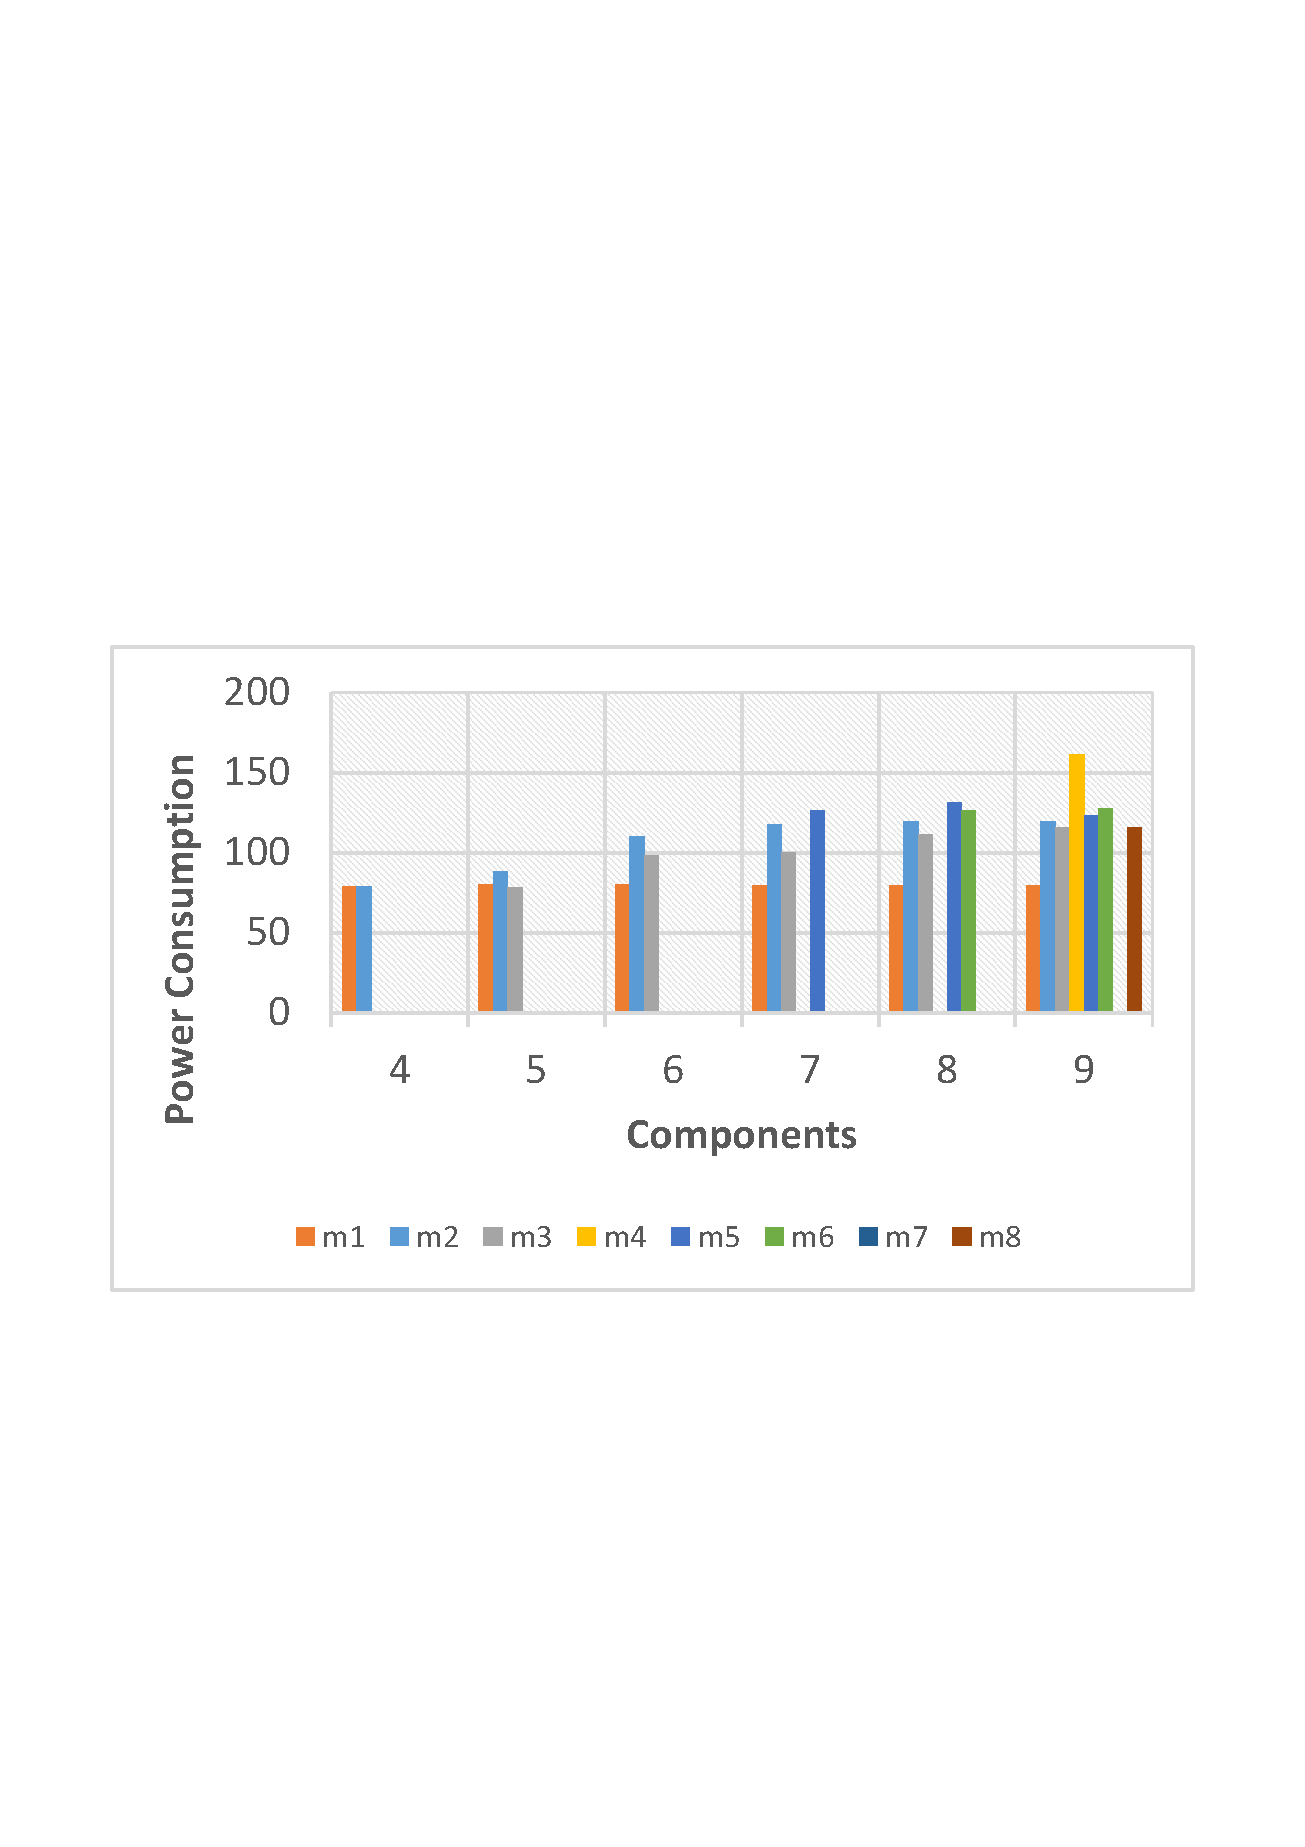
\includegraphics[width=0.45\textwidth]{images/power}
	} ~
	\subfloat[Computation times for software allocations. .\label{fig_computationtime_ilp}]{% 
		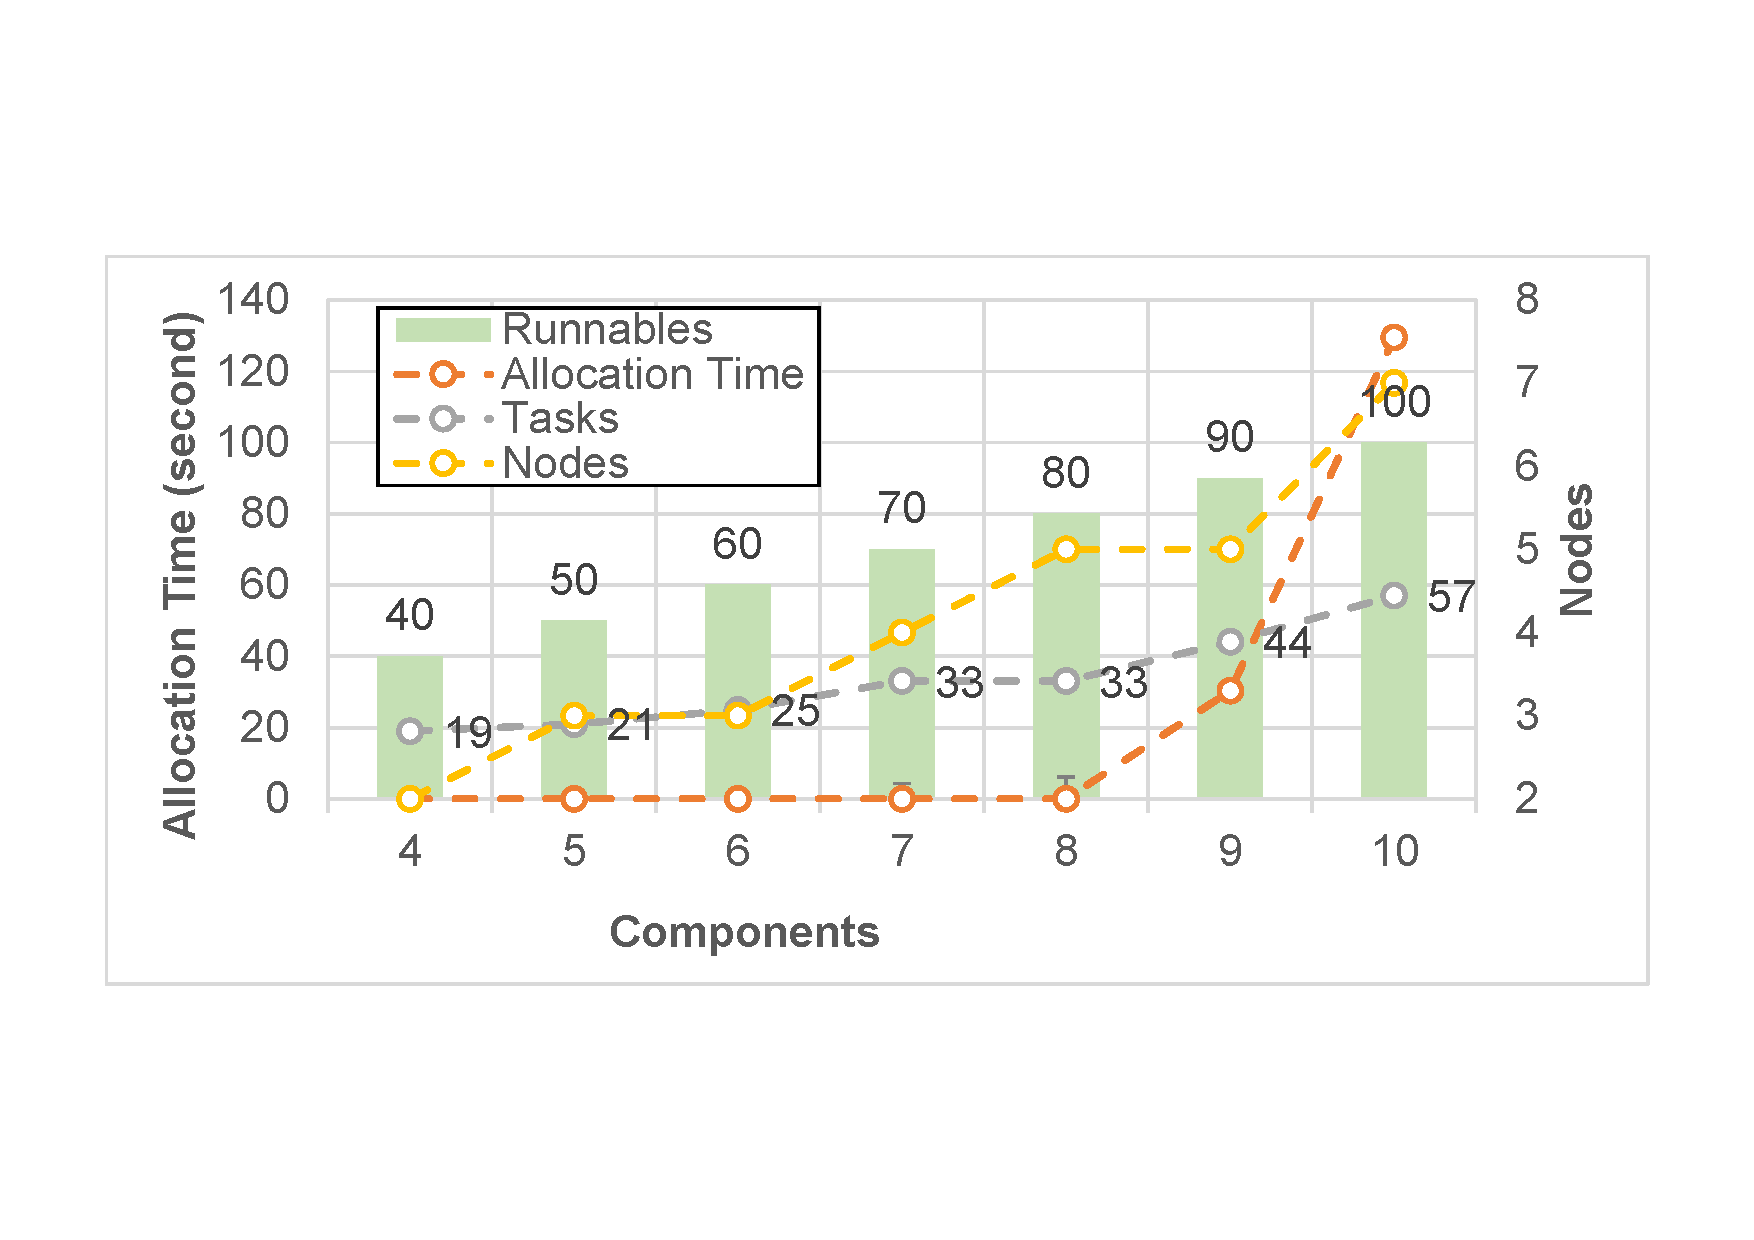
\includegraphics[width=0.55\textwidth]{images/increasing_components} 
	} 
	\caption{ILP optimization of different sizes of software applications based on the number of software components, cause-effect chains, computing nodes.} \label{fig_ilp_results}
\end{figure}

\noindent\textbf{The hybrid PSO approach validation: } we have prepared 7 software applications, which are identified by $\langle cimjgk\rangle$, where $c,m,g$, respectively, refer to the components, computing nodes and chains, and $i,j,k\in\mathbb{I}^+$, respectively, refer to the cardinality of $c,n,g$, respectively, in the application.

As opposed to the ILP approach, in this validation, we have to consider quality of the solutions since the solutions delivered by meta-heuristic algorithms do not guarantee optimality. Furthermore, we evaluate the impact of the proposed approximation algorithm to minimize the overhead of the replication on the optimization. 

Figure~\ref{fig_powerconsumption_ilp_metaheuristic} shows \ilp{} and all except \pso{} and \depso{} return optimal solutions in the first three problems. However, as the problem size increases, the hybrid PSO with the local search algorithms, i.e. \hcpso{} and \shpso{}, deliver better solutions as compared to \depso{}. 
% \begin{figure}
% 	\centering
% 	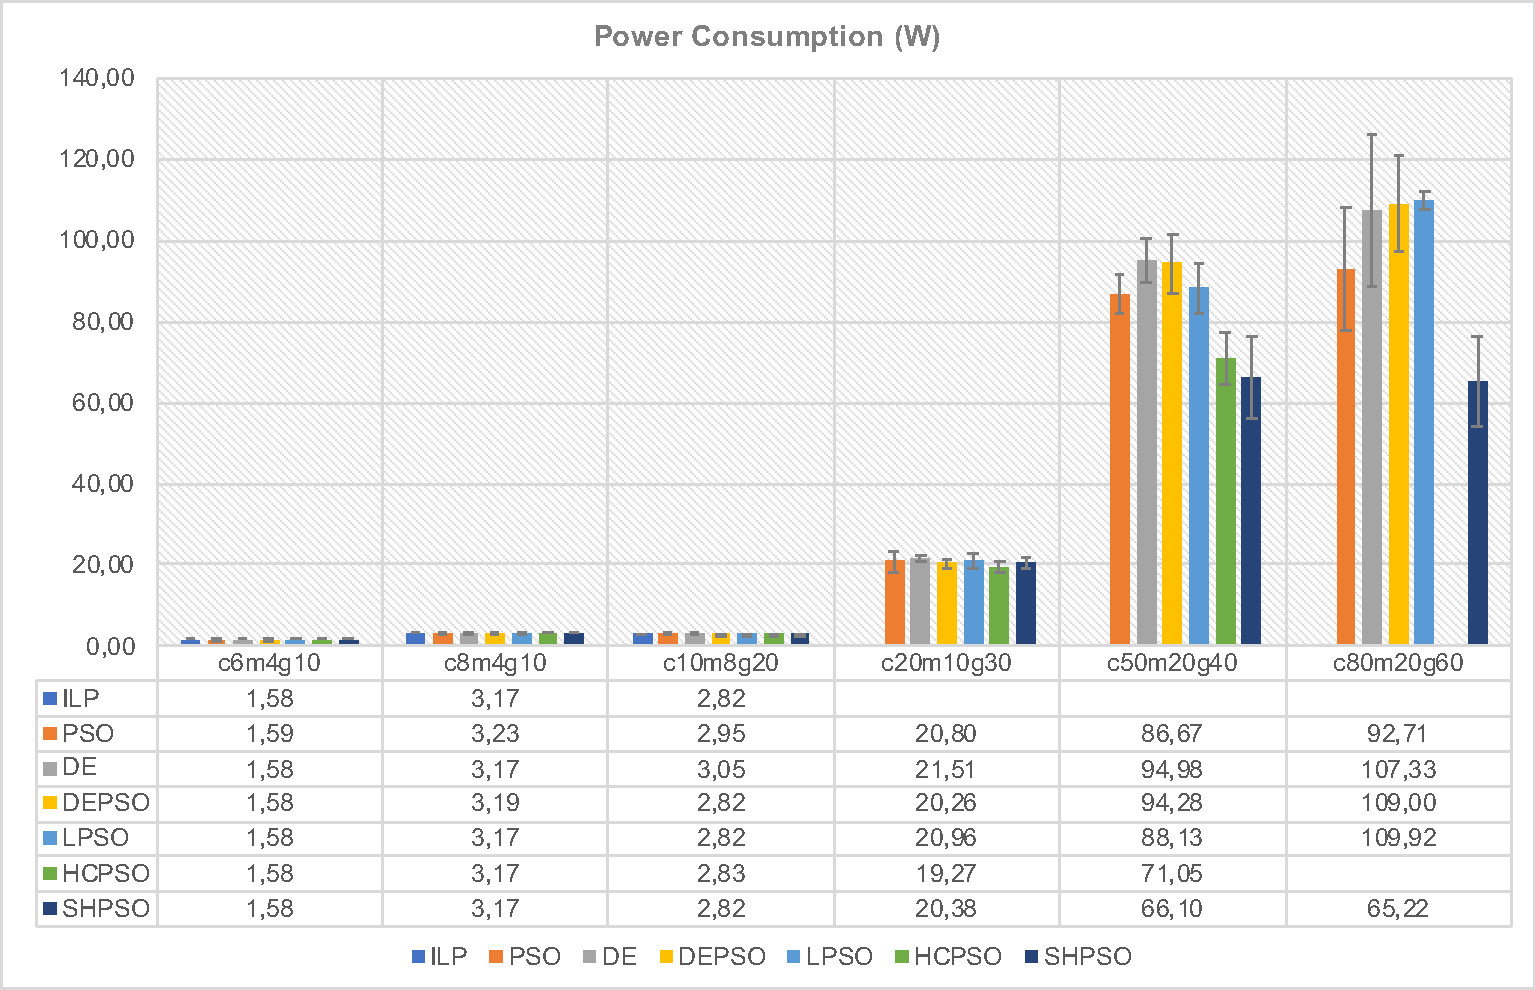
\includegraphics[width=0.8\linewidth]{images/power_consumption.pdf}
% 	\caption{Power consumption of nodes for different instances of software allocation problems by different optimization algorithms.}
% 	\label{fig_powerconsumption_ilp_metaheuristic}\vspace{-0.4cm}
% \end{figure}
\begin{center}
\resizebox {0.9\textwidth} {!} {
\begin{tikzpicture}[spy using outlines={circle,black,magnification=1.75,size=1.25cm, connect spies}]
\node {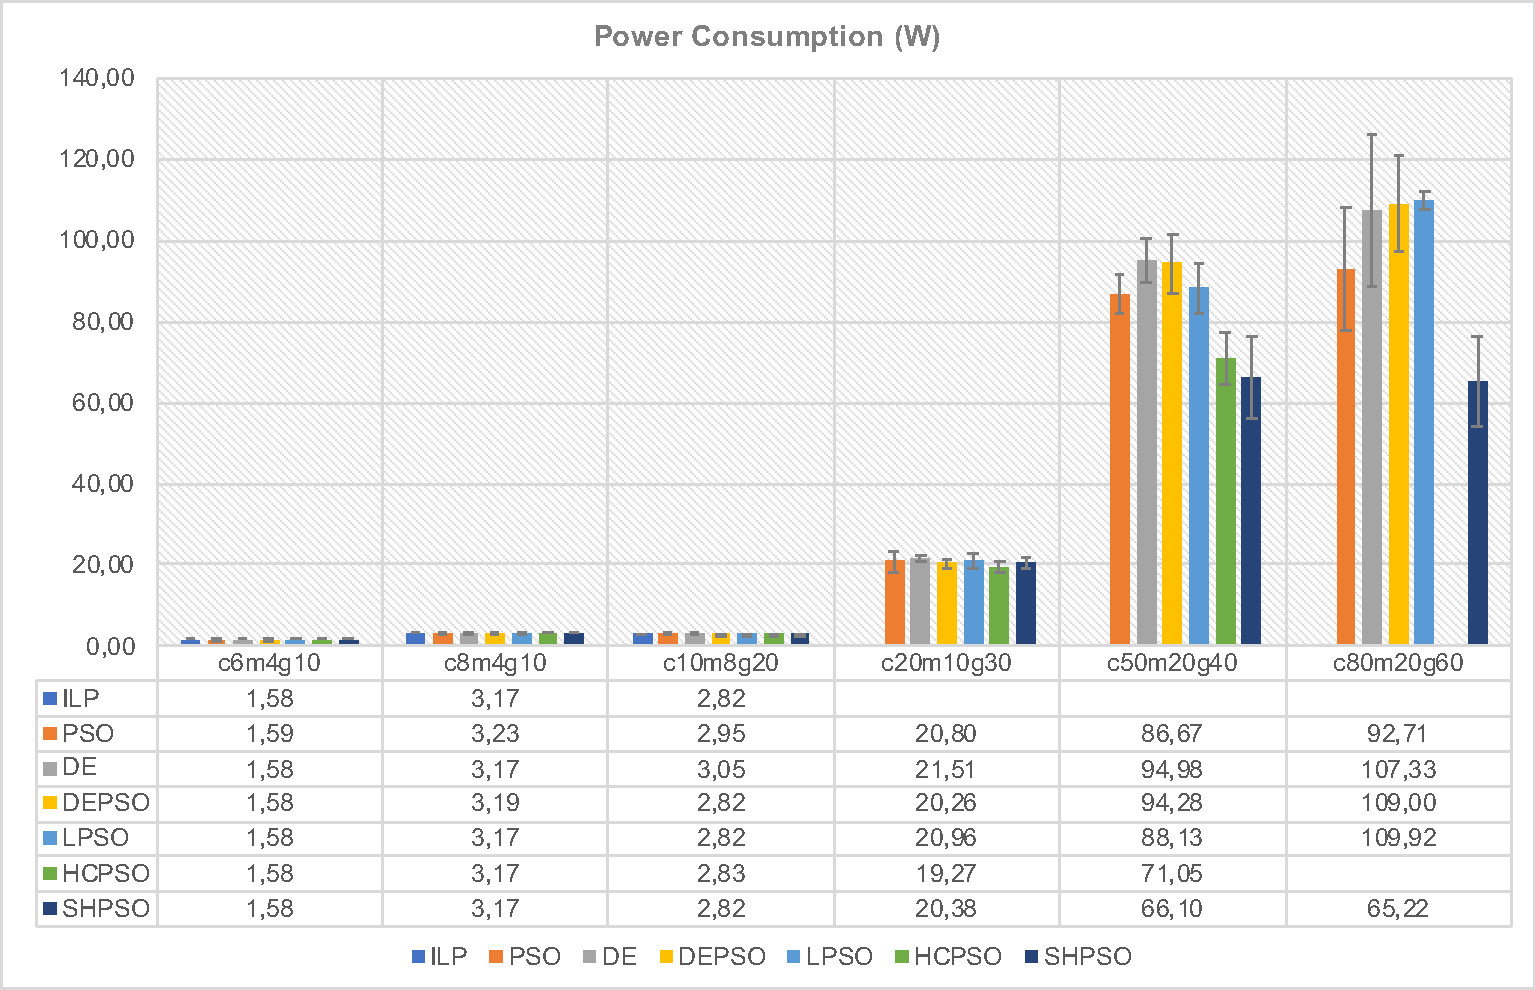
\includegraphics[width=1\linewidth]{images/power_consumption.pdf}};
\spy on (-2.1,-1.2) in node [draw,thin, ellipse, minimum width=9cm, minimum height=1.25cm,align=left] at (0,2.70);
\end{tikzpicture}}
\end{center}

Figure~\ref{fig_allocationtime_ilp_metaheuristic} shows that the hybrid \pso{} algorithms with local search perform the best in the last three problems except \hcpso{}, which fails to return near optimal solutions to the largest problem \pb{80}{20}{60} due to extremely large computation time, consequently manually interrupted. Thus, the stochastic version of the hill-climbing algorithm scales well, and its overall quality of the solution can be deemed acceptable as compared to \ilp{} or \hcpso. The analysis of the approximation algorithm that is introduced to lower the overhead of replication on the end-to-end computation has resulted in lower computation time, as expected, while impacting less the quality solutions. For more of the validation results and analysis, refer Paper F~\cite{Mahmud2019OptimizedConstraints}.
\begin{figure}[h]
	\centering
	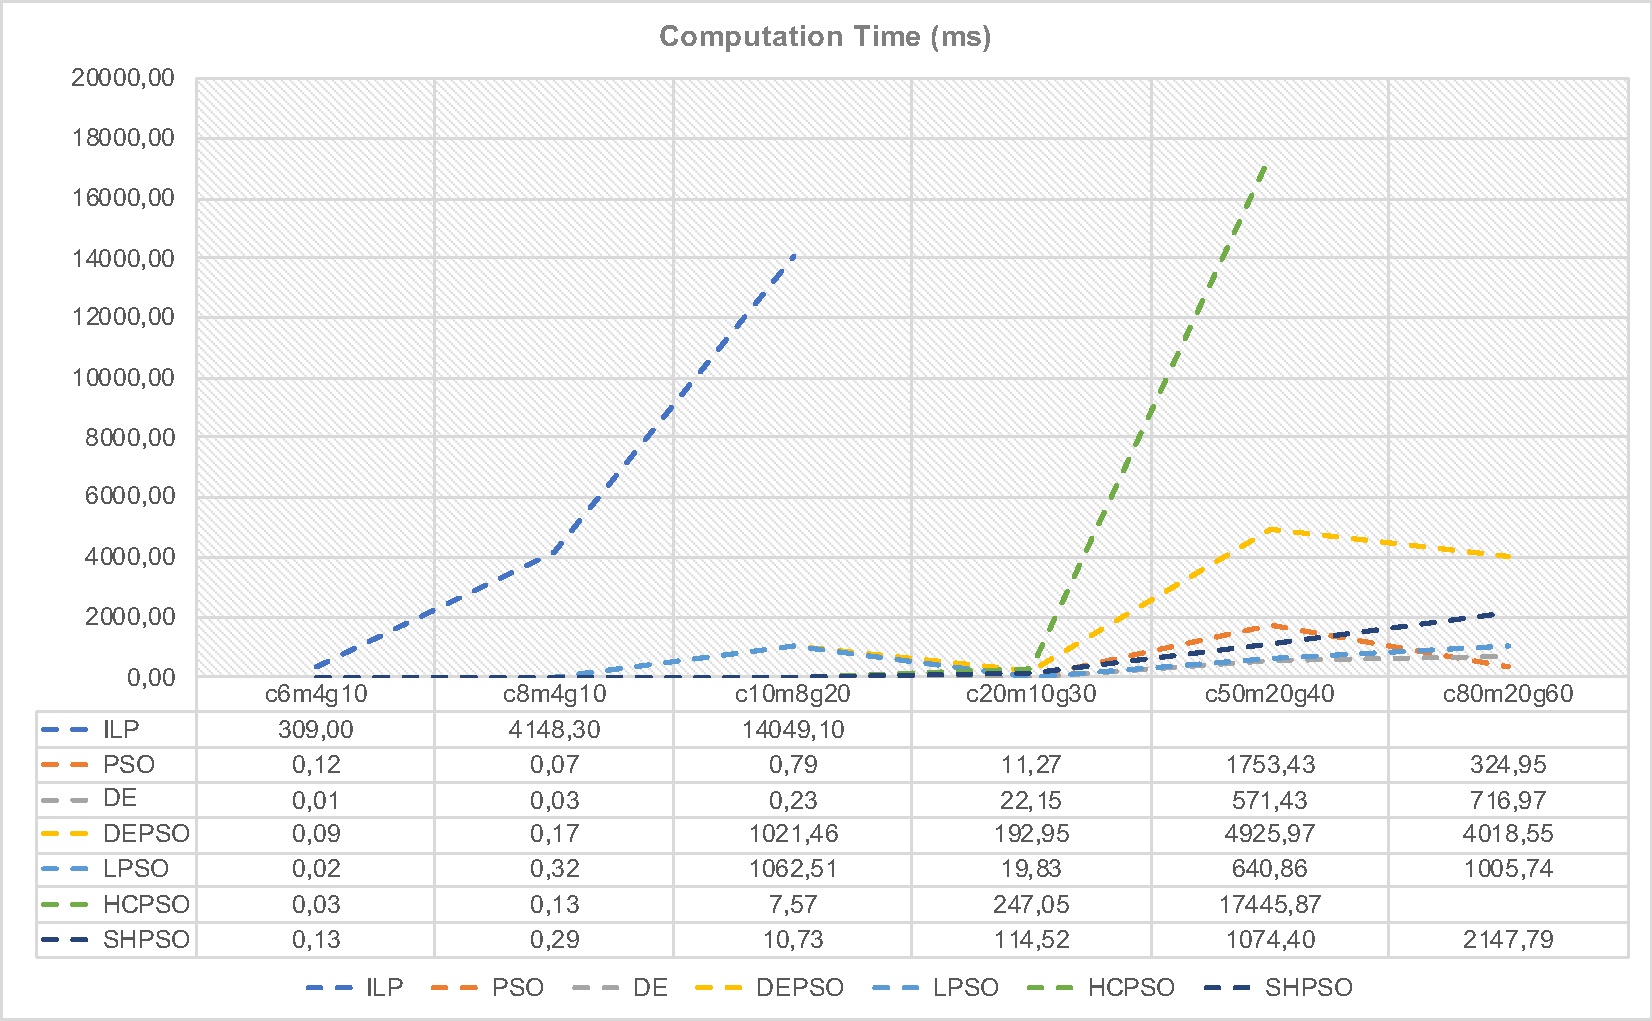
\includegraphics[width=0.9\linewidth]{images/time_summary.pdf}
	\caption{Computation time of the software allocation for different instances of the software allocation problems by different optimization algorithms.}
	\label{fig_allocationtime_ilp_metaheuristic}\vspace{-0.4cm}
\end{figure}

%Due to the replication of components to meet the reliability goals, the overhead of computing the delays is exponential. Figure~\ref{fig_chainsreplicationimprovements} compares the effect of with and without applying the approximation algorithm.  It shows that $61\%-81\%$ computation time improvement over the exact method while facing quality degradation only for samples $g_{30}d_{3}$ and  $g_{60}d_{2}$. The improvements are in seconds, which means for a single usage (or run) of the meta-heuristic optimization algorithms, it is not significant. However, considering practical engineering process, which requires several iterations, the commutative effect of applying the approximation algorithm can beneficial in terms of responsiveness to engineers. 
% \begin{figure}[h]
% 	\centering
% 	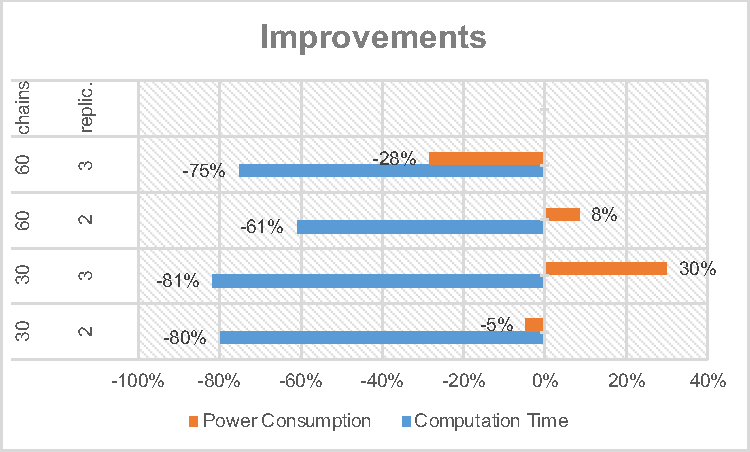
\includegraphics[width=0.7\linewidth]{images/chains_replication_improvements}
% 	\caption{Effect of approximate algorithm over delay calculations with replication.}
% 	\label{fig_chainsreplicationimprovements}
% \end{figure}

\section{Included Papers and their Mapping to Contributions and Goals}
\subsection*{Paper A}
ReSA: An ontology-based requirement specification language tailored to automotive systems. Nesredin~Mahmud, Cristina~Seceleanu and Oscar~Ljungkrantz.\textit{In the 10th IEEE International Symposium on Industrial Embedded Systems (SIES)(pp. 1-10). IEEE, 2015}.\label{lbl_resa}\\[6pt]
\textbf{Abstract:} \textit{Automotive systems are developed using multi-leveled architectural abstractions in an attempt to manage the increasing complexity and criticality of automotive functions. Consequently, well-structured and unambiguously specified requirements are needed on all levels of abstraction, in order to enable early detection of possible design errors. However, automotive industry often relies on requirements specified in ambiguous natural language, sometimes in large and incomprehensible documents. Semi-formal requirements specification approaches (e.g., requirement boilerplates, pattern-based specifications, etc.) aim to reduce requirements ambiguity, without altering their readability and expressiveness. Nevertheless, such approaches do not offer support for specifying requirements in terms of multi-leveled architectural concepts, nor do they provide means for early-stage rigorous analysis of the specified requirements. In this paper, we propose a language, called ReSA, which allows requirements specification at various levels of abstraction, modeled in the architectural language of EAST-ADL. ReSA uses an automotive systems' ontology that offers typing and syntactic axioms for the specification. Besides enforcing structure and more rigor in specifying requirements, our approach enables checking refinement as well as consistency of requirements, by proving ordinary boolean implications. To illustrate ReSA's applicability, we show how to specify some requirements of the Adjustable Speed Limiter, which is a complex, safety-critical Volvo Trucks user function.}\\[6pt]
\textbf{Personal Contributions: }I was the main driver of the paper. I developed the ReSA language including its syntax and semantics, and Cristina Seceleanu proposed a consistency analysis technique besides giving useful comments and ideas on the design of the language. Oscar Ljungkrantz provided useful materials from VGTT that were eventually analyzed for the language development, and gave feedback on the language design and implementation from an industrial viewpoint.\\
\textbf{Status:} Published

\subsection*{Paper B}
ReSA tool: Structured requirements specification and SAT-based consistency-checking. Nesredin~Mahmud, Cristina~Seceleanu and Oscar~Ljungkrantz. \textit{In the 2016 Federated Conference on Computer Science and Information Systems (FedCSIS)(pp. 1737-1746). IEEE, 2016.}\label{lbl_resatool}\\[6pt]
\textbf{Abstract:} \textit{Most industrial embedded systems requirements are
	specified in natural language, hence they can sometimes be
		ambiguous and error-prone. Moreover, employing an early-stage
		model-based incremental system development using multiple
		levels of abstraction, for instance via architectural languages
		such as EAST-ADL, calls for different granularity requirements
		specifications described with abstraction-specific concepts that
		reflect the respective abstraction level effectively.
		In this paper, we propose a toolchain for structured requirements
		specification in the ReSA language, which scales to multiple
		EAST-ADL levels of abstraction. Furthermore, we introduce
		a consistency function that is seamlessly integrated into the
		specification toolchain, for the automatic analysis of requirements
		logical consistency prior to their temporal logic formalization
		for full formal verification. The consistency check subsumes
		two parts: (i) transforming ReSA requirements specification into
		boolean expressions, and (ii) checking the consistency of the
		resulting boolean expressions by solving the satisfiability of their
		conjunction with the Z3 SMT solver. For validation, we apply
		the ReSA toolchain on an industrial vehicle speed control system,
		namely the Adjustable Speed Limiter.}\\[6pt]%abstract
	\textbf{Personal Contributions: }I was the main driver of the paper. I developed the ReSA toolchain that consists of the editor and the consistency checker including the integration with the Z3 SAT solver in the backend. Cristina Seceleanu formulated the consistency checking and together with Oscar Ljungkrantz, they contributed to the paper with useful comments and ideas.\\
		\textbf{Status: }Published

\subsection*{Paper C}
	Specification and semantic analysis of embedded systems requirements: From description logic to temporal logic. Nesredin~Mahmud, Cristina~Seceleanu and Oscar~Ljungkrantz. \textit{In the International Conference on Software Engineering and Formal Methods (SEFM)(pp. 332-348). Springer, Cham, 2017.}\label{lbl_resadl}\\[6pt]%authors
	\textbf{Abstract:} \textit{Due to the increasing complexity of embedded systems, early detection of software/hardware errors has become desirable. In this context, effective yet flexible specification methods that support rigorous analysis of embedded systems requirements are needed. Current specification methods such as pattern-based, boilerplates normally lack meta-models for extensibility and flexibility. In contrast, formal specification languages, like temporal logic, Z, etc., enable rigorous analysis, however, they usually are too mathematical and difficult to comprehend by average software engineers. In this paper, we propose a specification representation of requirements, which considers thematic roles and domain knowledge, enabling deep semantic analysis. The specification is complemented by our constrained natural language specification framework, ReSA, which acts as the interface to the representation. The representation that we propose is encoded in description logic, which is a decidable and computationally-tractable ontology language. By employing the ontology reasoner, Hermit, we check for consistency and completeness of requirements. Moreover, we propose an automatic transformation of the ontology-based specifications into Timed Computation Tree Logic formulas, to be used further in model checking embedded systems.}\\[6pt]%abstract
	\textbf{Personal Contributions:} I was the main driver of the language. I developed the ReSA language semantics using event-base approach, which is encoded in description logic. Cristina~Seceleanu and Ljungkrantz~Oscar provided with useful ideas and comments.\\
	\textbf{Status:} Published

\subsection*{Paper D}
SIMPPAAL - A Framework For Statistical Model Checking of Industrial Simulink Models. Predrag~Filipovikj, Nesredin~Mahmud, Raluca~Marinescu, Cristina~Seceleanu, Oscar~Ljungkrantz and Henrik~L\"{o}nn. \textit{Submitted to ACM Transactions on Software Engineering and Methodology (TOSEM).}\label{lbl_simulink_ilp}
\\[3pt]{\footnotesize This article is an extended version of the following conference paper:
     Simulink to UPPAAL Statistical Model Checker: Analyzing Automotive Industrial Systems.
Predrag Filipovikj, Nesredin Mahmud, Raluca Marinescu, Cristina Seceleanu, Oscar Ljungkrantz, Henrik L{\"o}nn. In Proceedings of the 21st International
Symposium on Formal Methods (FM2016), pages 748-756. Limassol, Cyprus. Springer, LNCS, November 2016. Revisions required. }\\[6pt]%authors
	\noindent \textbf{Abstract:} \textit{The evolution of automotive systems has been rapid. Nowadays, electronic brains control dozens of functions in vehicles, like
		braking, cruising, etc. Model-based design approaches, in environments such as MATLAB Simulink, seem to help in addressing
		the ever-increasing need to enhance quality, and manage complexity, by supporting functional design from a set of block
		libraries, which can be simulated and analyzed for hidden errors, but also used for code generation. For this reason, providing
		assurance that Simulink models fulfill given functional and timing requirements is desirable. In this paper, we propose a
		pattern-based, execution-order preserving automatic transformation of atomic and composite Simulink blocks into stochastic
		timed automata that can then be formally analyzed with Uppaal Statistical Model Checker (Uppaal SMC). To enable this, we
		first define the formal syntax and semantics of Simulink blocks and their composition, and show that the transformation is
		provably correct for a certain class of Simulink models. Our method is supported by the SIMPPAAL tool, which we introduce
		and apply on two industrial Simulink models, a prototype called the Brake-by-Wire and an operational Adjustable Speed
		Limiter system. This work enables the formal analysis of industrial Simulink models, by automatically generating stochastic
		timed automata counterparts.}\\[6pt]%abstract
	\textbf{Personal Contributions: } The three co-authors contributed equally to writing the paper. Technically, I equally contributed with proposing the pattern-based semantics of Simulink blocks, together with Predrag Filipovikj. I introduced a mechanism to enforce the execution order of the blocks using inter-arrival times. Predrag implemented the flattening algorithm and the tool for the automatic transformation of Simulink models into a network of timed automata with stochastic semantics. Raluca Marinescu contributed with analyzing the BBW system, Cristina Seceleanu contributed with defining the methodology, and with useful ideas and comments. Guillermo Rodriguez-Navas wrote the related work section. The industrial coauthors provided the use cases and commented on the final draft.\\
	\noindent\textbf{Status:} Revisions required. 

\subsection*{Paper E}
Power-aware Allocation of Fault-tolerant Multirate AUTOSAR Applications.
     Nesredin~Mahmud, Guillermo~Rodriguez-Navas, Hamid~Faragardi, Saad~Mubeen and Cristina~Seceleanu. \textit{In the 25th Asia-Pacific Software Engineering Conference (APSEC'18). IEEE.}  
     \label{lbl_softwareallocation_ilp}
\\[6pt]%authors
\textbf{Abstract:} \textit{The growing complexity of automotive functionality has attracted revolutionary computing architectures such as mixed-criticality design, which enables effective consolidation of software applications with different criticality on a shared execution platform. Mixed-critical design that is required to satisfy end-to-end timing and reliability specifications should consider power-efficient software design in order to accommodate more and more functionality. Due to the recursive and exhaustive nature of the real-time and reliability analysis, exact methods, e.g., branch and bound, dynamic programming, are prohibitively expensive. We propose hybrid particle-swarm optimization algorithms based on differential evolution and hill-climbing algorithms to minimize power consumption of the safety-critical software, which have end-to-end timing and reliability requirements, on a network of heterogeneous computing units. The optimization approach employs fault tolerance to maximize reliability of the software applications subsequently meet the reliability requirements. Our proposed integrated software-allocation approach is evaluated using a range of synthetic software applications based a real-world automotive benchmark. The evaluation makes comparative analysis of the differential evolution, particle-swarm optimization, integer-linear programming and hybrid particle-swarm optimization algorithms. The results show that the hybrid algorithms based on the hill-climbing algorithms outperform the rest of the meta-heuristic algorithms, in particular, the stochastic version of the hill-climbing algorithm scales well in large software allocation optimization problems while its overall optimality performance can be deemed acceptable.
}\\[6pt]%abstract
\textbf{My Contributions: } I was the main driver of the paper. I developed the system model with the guidance of the co-authors, and formulated the optimization problem with the guidance of Hamid~Faragardi, implemented the the problem in Java, and collected and analyzed the experimental results. The co-authors gave writing updates, useful ideas and comments on the paper, and specifically: Guillermo~Rodriguez-Navas on reliability analysis, Hamid~Faragardi on optimization, Saad~Mubeen on the timing analysis and Cristina~Seceleanu on the objective function and constraints.\\
\textbf{Status:} Published

\subsection*{Paper F}
Optimized Allocation of Fault-tolerant Embedded Software with End-to-end Timing Constraints.	\textit{M\"{a}lardalen Real-time Research Center Technical Report (MRTC), ISRN MDH-MRTC-325/2019-1-SE, 2019}. Submitted to Elsevier Journal of Systems Architecture (JSA).\\[6pt]%authors
\textbf{Abstract:} \textit{It is desirable to optimize power consumption of distributed safety-critical software that realize fault tolerance and maximize reliability as a result, to support the increasing complexity of software functionality in safety-critical embedded systems. Likewise, safety-critical applications that are required to meet end-to-end timing constraints may require additional computing resources. In this paper, we propose a scalable software-to-hardware allocation based on hybrid particle-swarm optimization with hill-climbing and differential algorithms to efficiently map software components to a network of heterogeneous computing nodes while meeting the timing and reliability constraints. The approach assumes fixed-priority preemptive scheduling, and delay analysis that value freshness of data, which is typical in control software applications.
Our proposed solution is evaluated on a range of software applications, which are synthesized from a real-world automotive AUTOSAR benchmark. The evaluation makes comparative analysis of the different algorithms, and a solution based on integer-linear programming, which is an exact method. The results show that the hybrid with the hill-climbing algorithms return very close solutions to the exact method and outperformed the hybrid with the differential algorithm, though consumes more time. The hybrid with the stochastic hill-climbing algorithm scales better and its optimality can be deemed acceptable.}\\[6pt]%abstract
\textbf{Personal Contributions: } I was the main driver of the paper. I developed the system model with the guidance of the co-authors, and formulated the optimization problem with the guidance of Hamid~Faragardi, implemented the the problem in Java, and collected and analyzed the experimental results. The co-authors gave writing updates, useful ideas and comments on the paper, and specifically: Guillermo~Rodriguez-Navas on reliability analysis, Hamid~Faragardi on optimization, Saad~Mubeen on the timing analysis and Cristina~Seceleanu on the objective function and constraints. \\%my contribution
\textbf{Status:} Submitted to Journal of System Architecture (JSA), Elsevier Journals.\\


In summary, the mapping between the included papers and the research contributions is given in Table~\ref{paper_contribution}, whereas the mapping between the research contributions and the research goals is given in Table~\ref{contribution_goals}.

% Please add the following required packages to your document preamble:
% \usepackage{booktabs}
\begin{table}[h!]
\centering
 \rowcolors{2}{gray!25}{white}
	\begin{tabular}{@{}ccccc@{}}
	%\rowcolor{gray!50}
		\toprule
		Paper & RC1 & RC2& RC3 & RC4\\ \midrule
		Paper A & $\times$ &  &  &  \\
		Paper B & $\times$ & $\times$ &  &  \\
		Paper C &  & $\times$ &  &  \\
		Paper D &  &  & $\times$  &\\
		Paper E &  &  &  & $\times$ \\
		Paper F &  &  &  & $\times$\\ \bottomrule
	\end{tabular}
\caption{Mapping between the included papers and the research contributions.}\label{paper_contribution}
\end{table}

% Please add the following required packages to your document preamble:
% \usepackage{booktabs}
\begin{table}[h!]
\centering
 \rowcolors{2}{gray!25}{white}
		\begin{tabular}{@{}cccccc@{}}
	%\rowcolor{gray!50}
		\toprule
		Contribution & RG1 & RG2& RG3 & RG4 & RG5\\ \midrule
		RC1 & $\times$ &  &  &  &$\times$\\
		RC2 &  & $\times$ &  & & $\times$\\
		RC3 &  &  & $\times$ & & $\times$\\
		RC4 &  &  &  & $\times$ &$\times$\\\bottomrule
	\end{tabular}
\caption{Mapping between the research contributions and the research goals.}\label{contribution_goals}
\end{table}
